% Attention: Font "FiraCode N(erd) F(ont)" have different name between macOS and windows

%!TEX encoding = UTF-8 Unicode
\documentclass[a4paper,UTF8,heading=false,12pt]{article}
\usepackage[heading = false]{ctex}
\usepackage{graphicx}

% package
\usepackage{xeCJK}
\usepackage{blindtext}
\usepackage{palatino}
% \usepackage{titlesec}
\usepackage{needspace}
\usepackage[toc,page]{appendix}
\usepackage{metainfo}
\usepackage[pagestyles,raggedright]{titlesec}
\usepackage[xetex,colorlinks=false,hidelinks,pdfstartview=FitV]{hyperref}
\usepackage{amsmath,amssymb}
\usepackage{newpxtext,newpxmath}
\usepackage{listings}
\usepackage{fontspec}
\usepackage{xcolor-material}
\usepackage{enumitem}
\usepackage{booktabs}
% configuration
\fontsize{16pt}{\baselineskip}
%\setmonofont{FiraCode NF}
\CJKfamily{zhsong}
%\addtolength{\parindent}{3cm}
% code configuration
\definecolor{codegreen}{rgb}{0,0.6,0}
\definecolor{codegray}{rgb}{0.5,0.5,0.5}
\definecolor{codepurple}{rgb}{0.58,0,0.82}
\definecolor{backcolour}{rgb}{0.95,0.95,0.92}
\lstdefinestyle{customc}{
    belowcaptionskip=1\baselineskip,
    breaklines=true,
    frame=none,
    xleftmargin=2em,
    language=C++,
    showstringspaces=false,
    basicstyle=\footnotesize\ttfamily,
    keywordstyle=\bfseries\color{green!40!black},
    commentstyle=\itshape\color{purple!40!black},
    numberstyle=\fontspec{FiraCode NF}\color{darkgray},
    numbers=left,
    identifierstyle=\color{blue},
    stringstyle=\color{orange},
}

\usepackage[paperwidth=210mm, paperheight=297mm, margin=20 mm]{geometry}

\newcommand\subtitle[1]{{\small #1}} 

\begin{document}
\title{
    数据库系统概论实验报告 \\
    \subtitle{实验四: 两种方式向数据表添加、导入和导出数据}
}
\author{陈羿羽 \thanks{陈羿羽:西南大学2019级计算机科学与技术4班 - 222019603193014}}
\maketitle

\begin{abstract}
    本次实验的目标为:
    \begin{enumerate}
        \item 使用数据库管理系统SQL Server 或者MySQL操作数据库。
        \item 掌握创建、查看、修改和删除数据表的基本操作。
    \end{enumerate}
\end{abstract}

\newpage

\section{实验准备}

\begin{enumerate}
    \item 一台PC机或笔记本电脑
    \item 能够上网
\end{enumerate}

\section{实验要求}

\begin{enumerate}
    \item 查资料观看数据库管理系SQL Server 或者MySQL的数据表数据添加、导入和导出视频。
    \item 使用视图方式和命令方式向数据表添加、导入和导出数据。
    \item 学习了解数据表字段的基本类型。
\end{enumerate}

\section{实验内容}

\subsection{视图方式建立数据表}

向实验三创建的数据表添加数据:

\subsubsection{文件方式导入数据}

自己各构造10条存在名字为“学生成绩.txt”和“班级信息.txt”的文本文件中,然后导入到数据库响应\footnote{"响应表"是"相应"的表吗,并没有数据库响应表这玩意}表中。(其中涉及姓名的信息要有一条和自己的姓名相关的信息)

\newpage

此处我们构造了十条学生成绩信息记录与班级信息记录,如下图1和图2所示,其中学生成绩信息记录为制表符格式的文本文件,班级信息记录为逗号分隔符格式的文本文件。

\begin{figure}[htbp]
    \centering
    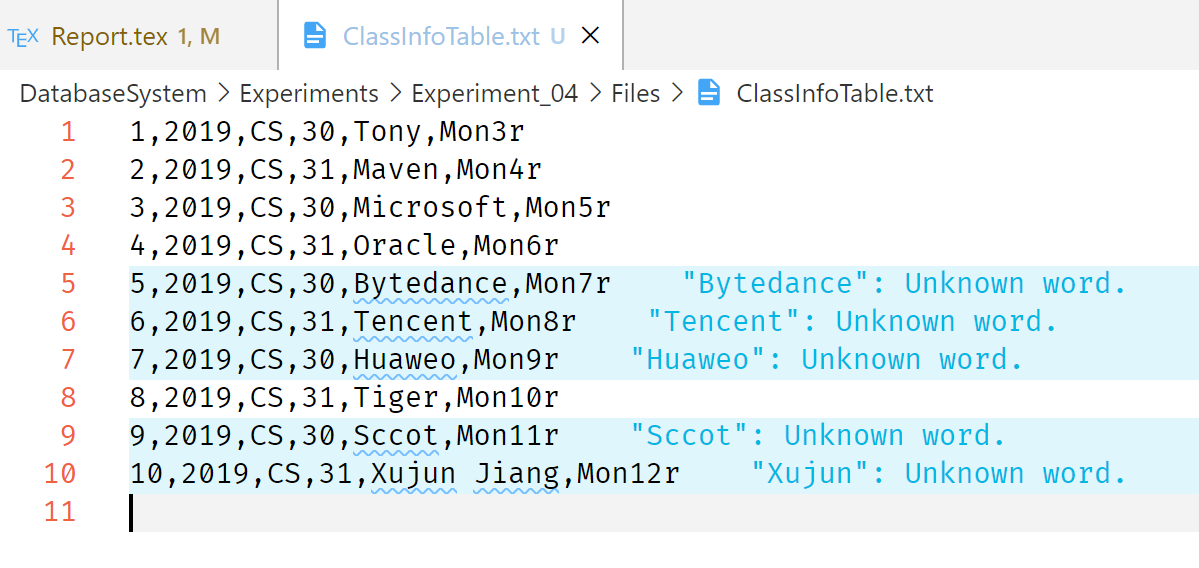
\includegraphics[width=10cm]{../Images/ClassInfoTable.png}
    \caption{生成的班级信息文件,命名为ClassInfoTable.txt}
\end{figure}

\begin{figure}[htbp]
    \centering
    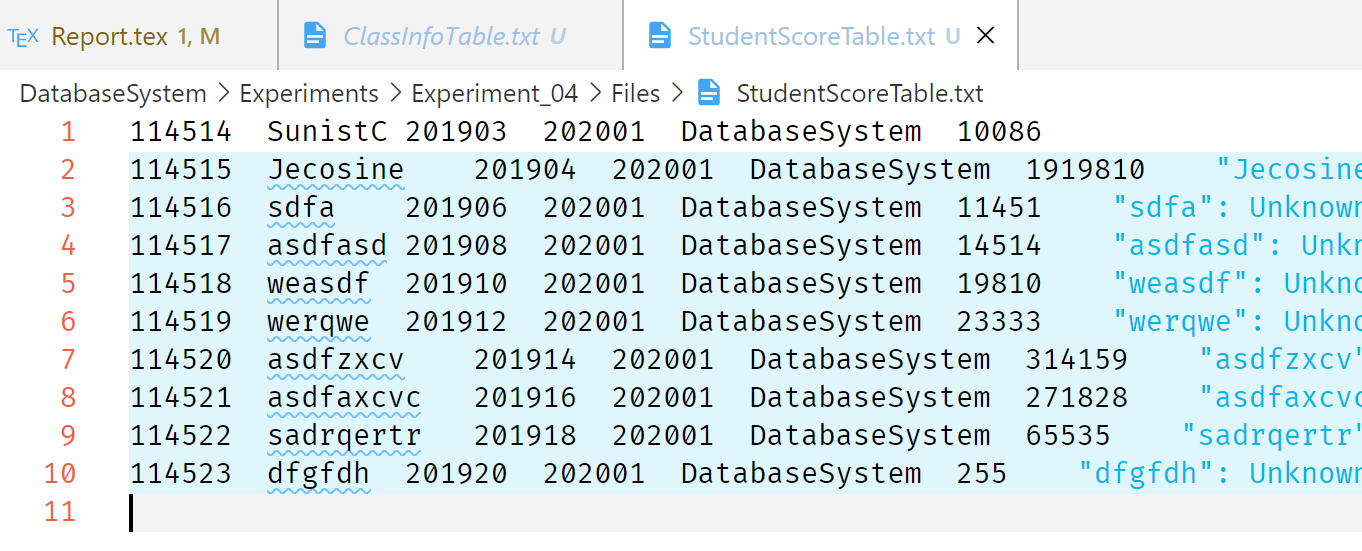
\includegraphics[width=10cm]{../Images/StudentScoreTable.png}
    \caption{生成的学生成绩信息文件,命名为StudentScoreTable.txt}
\end{figure}

\newpage

然后我们将其添加到我们的数据库中,其中,班级信息表我们选用"Comma-separated"模式导入,学生成绩信息表我们选用"Tab-separated"模式导入,如下图3和图4所示,导入结果如下图5和图6所示。

\begin{figure}[htbp]
    \centering
    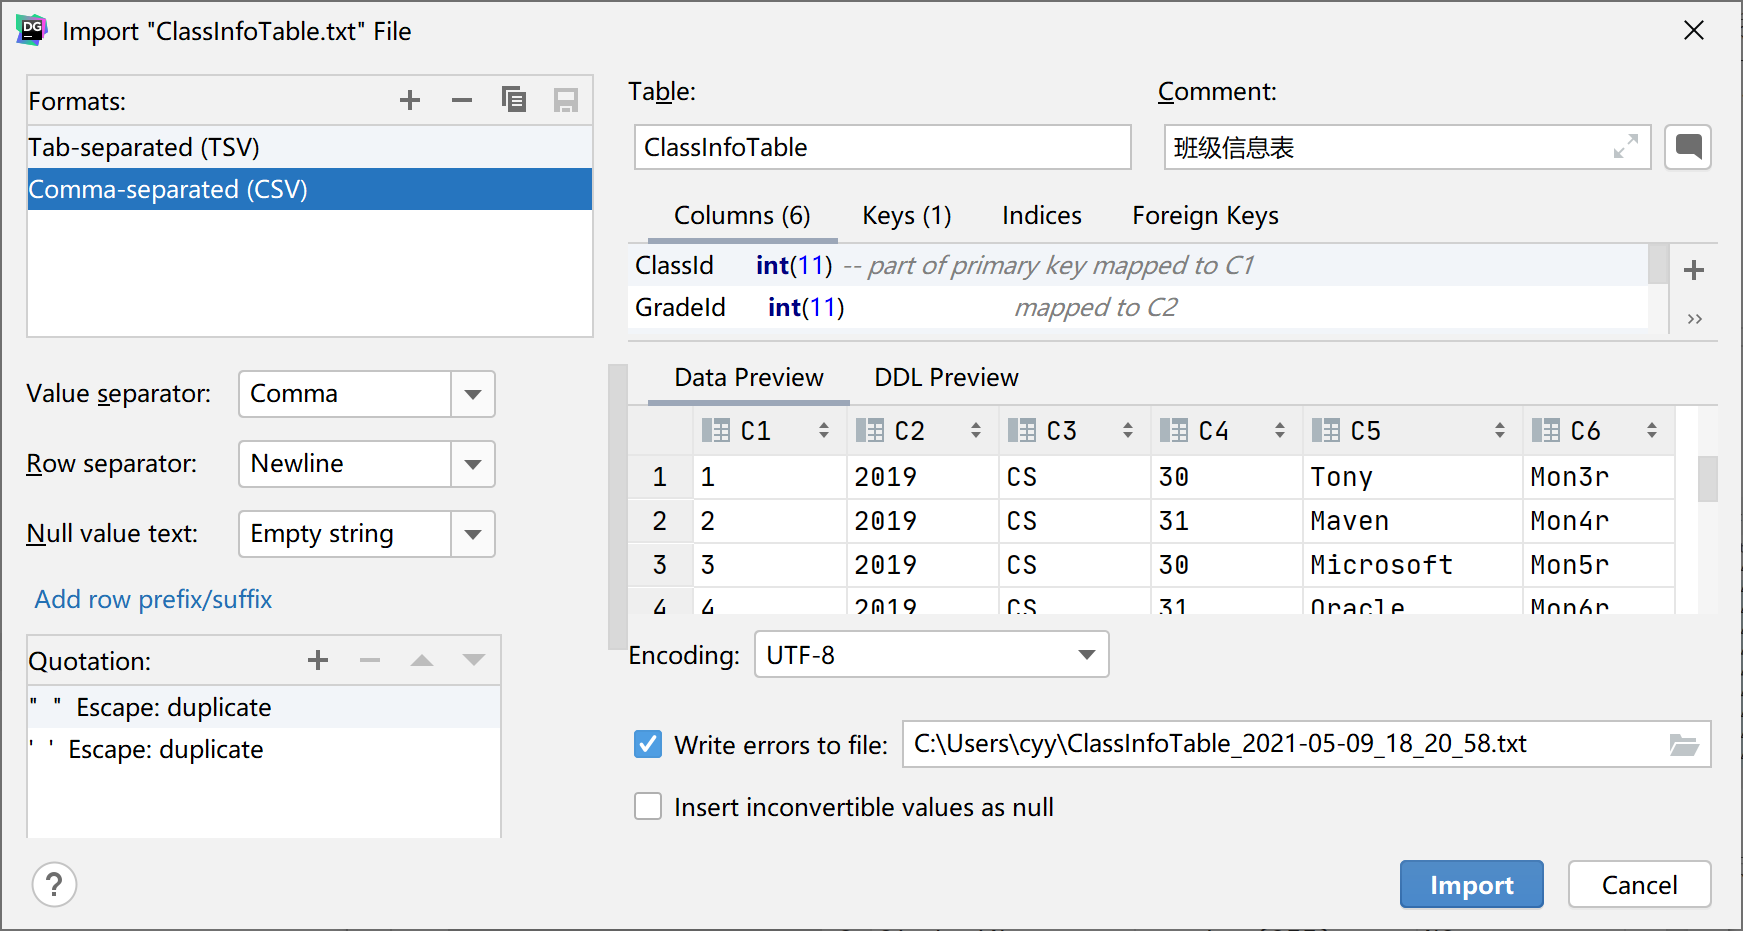
\includegraphics[width=15cm]{../Images/ClassInfoTable_OnImport.png}
    \caption{使用"Comma-separated"模式导入班级信息表}
\end{figure}

\begin{figure}[htbp]
    \centering
    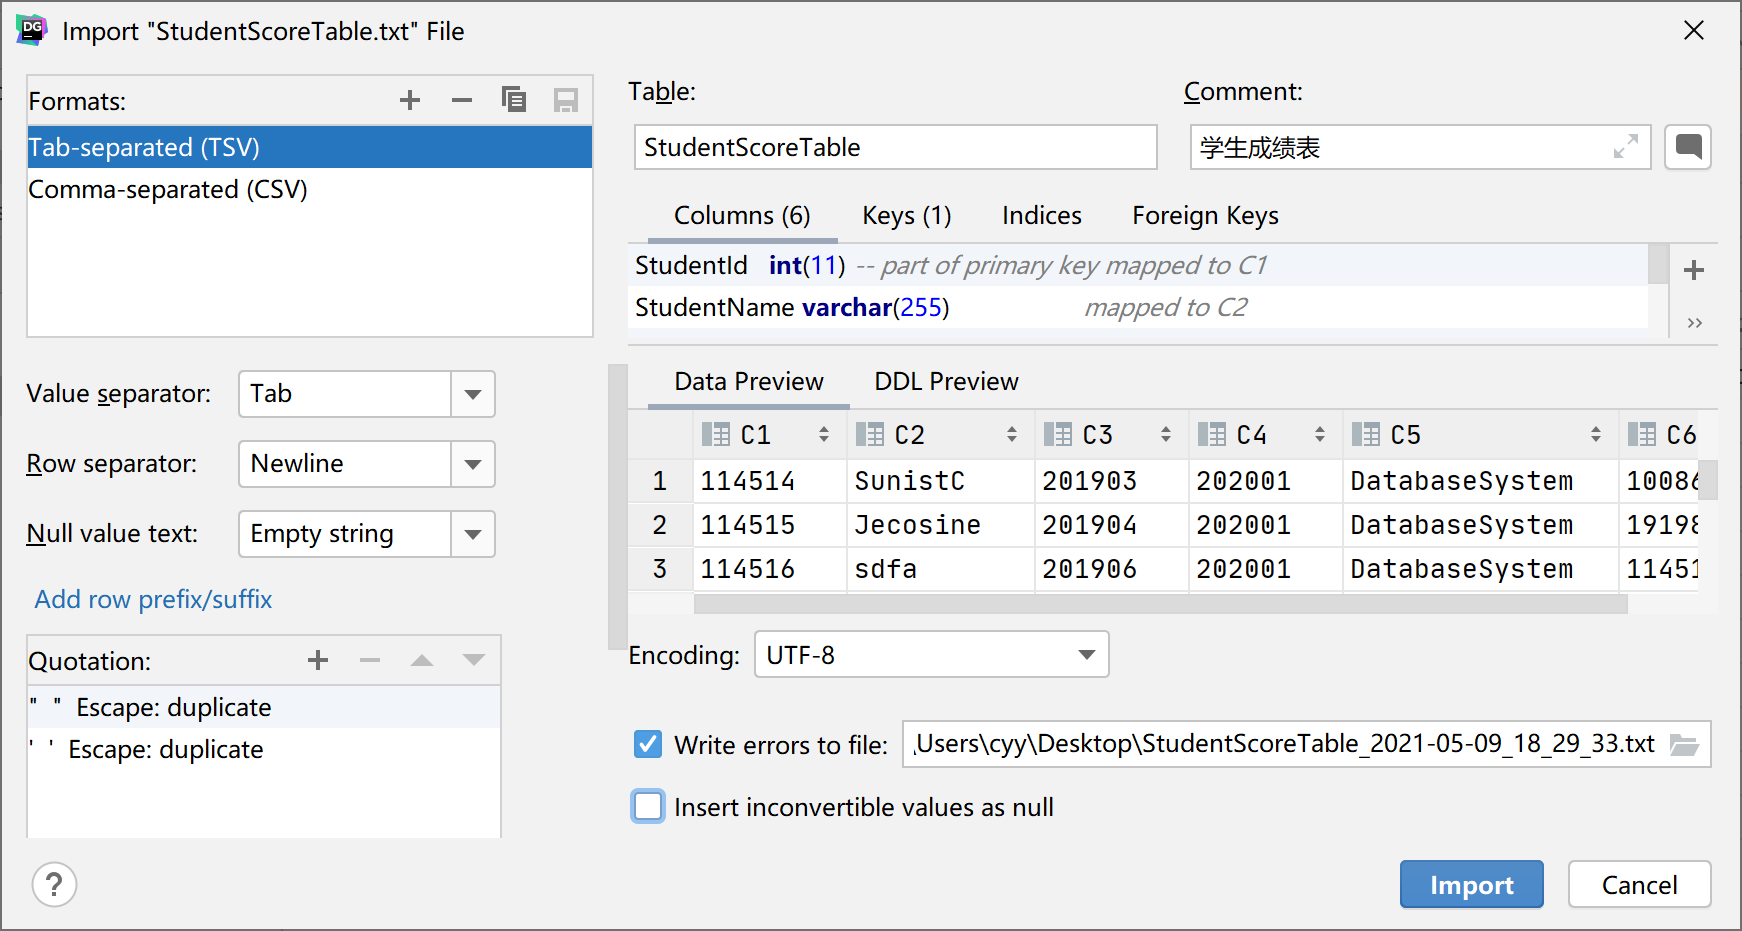
\includegraphics[width=15cm]{../Images/StudentScoreTable_OnImport.png}
    \caption{使用"Tab-separated"模式导入学生成绩信息表}
\end{figure}

\begin{figure}[htbp]
    \centering
    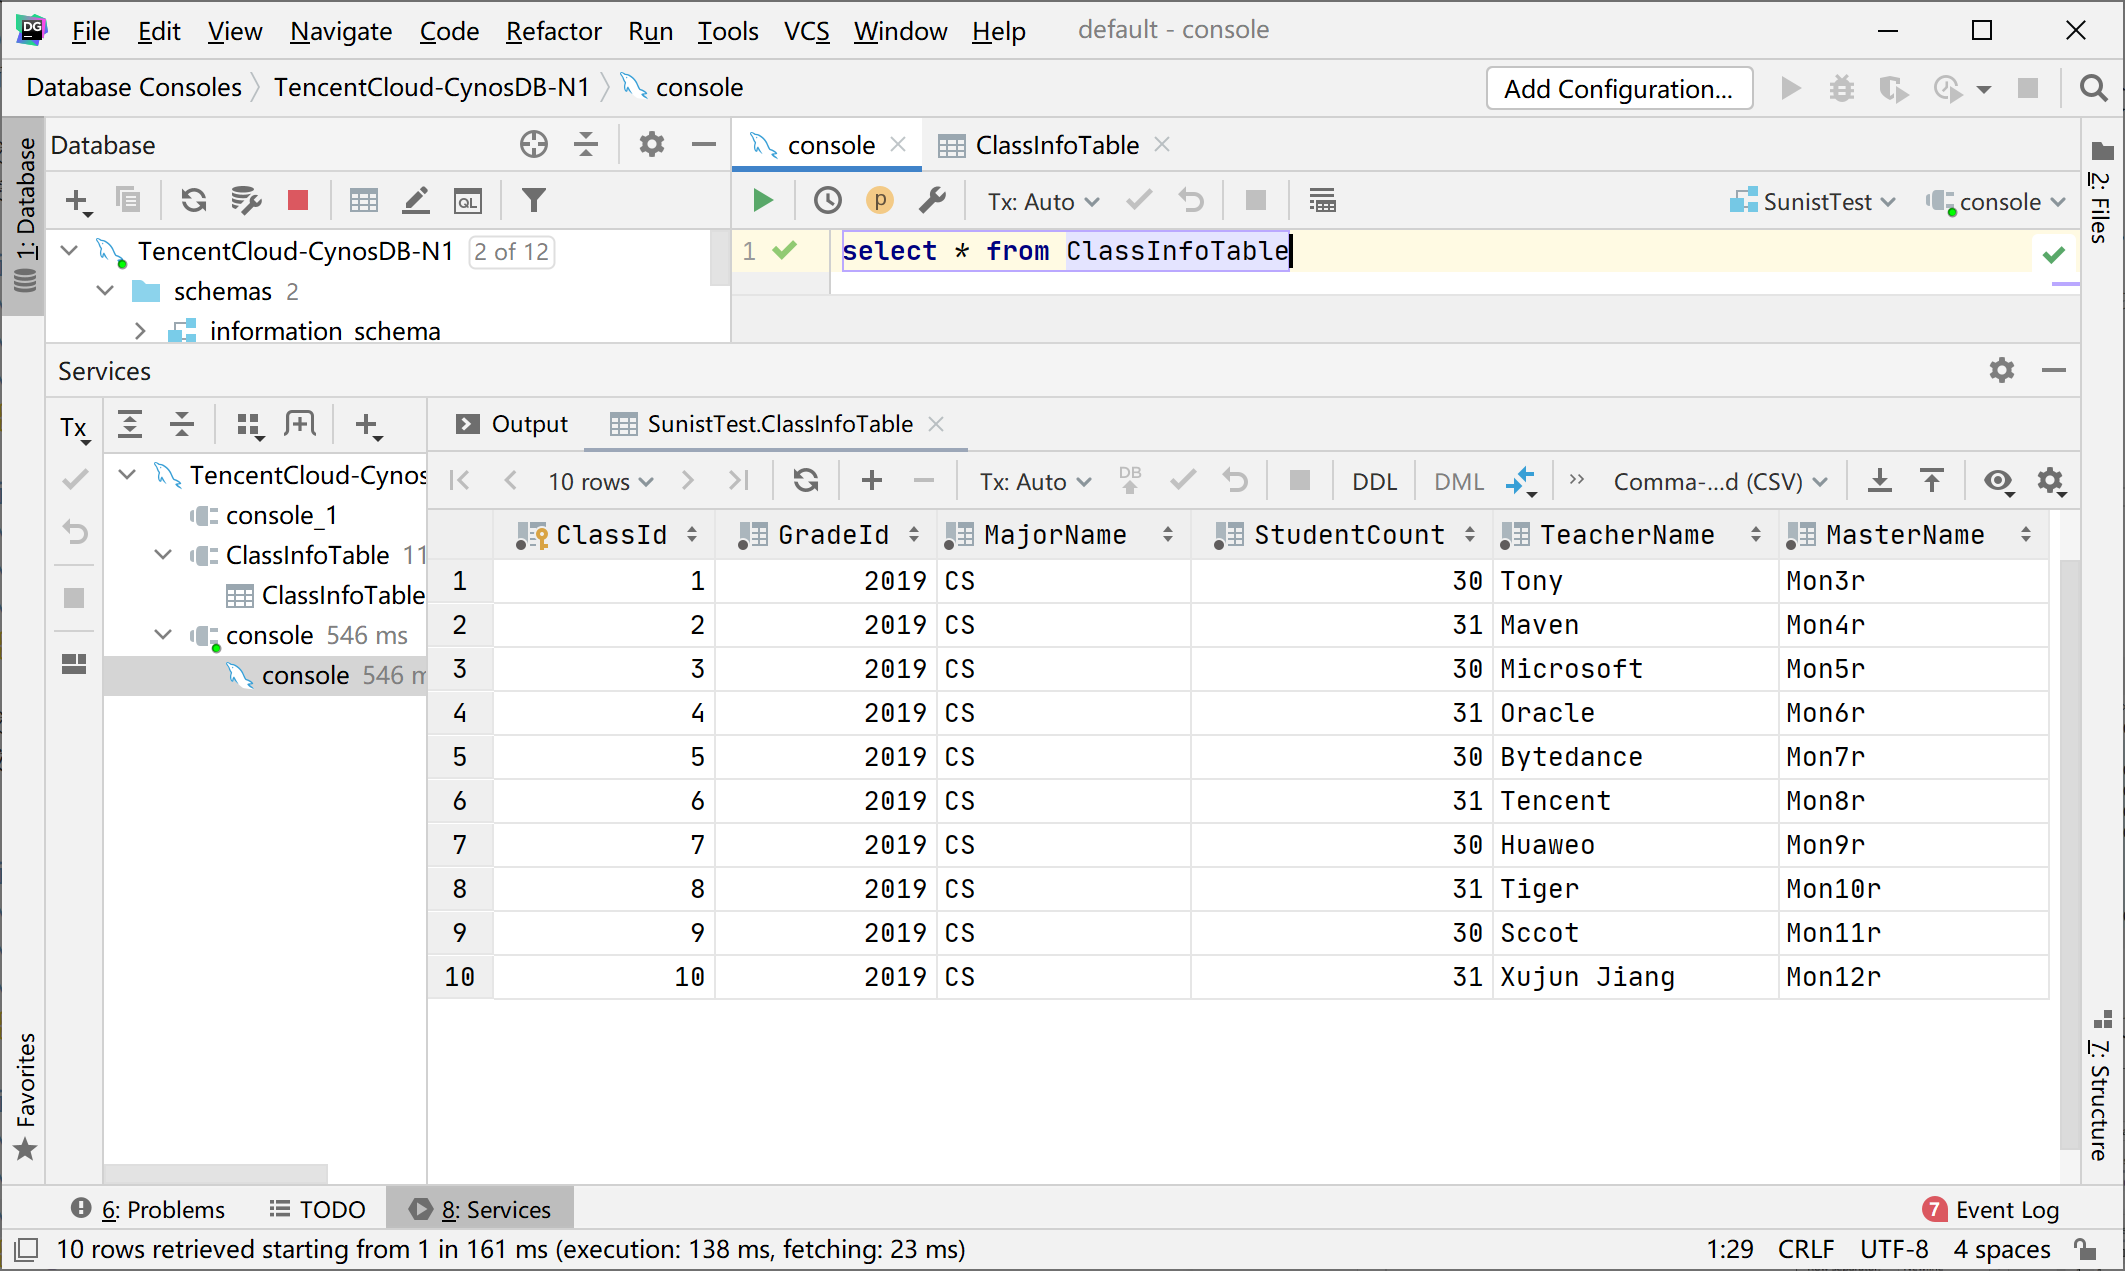
\includegraphics[width=15cm]{../Images/ClassInfoTable_OnImported.png}
    \caption{导入完成的班级信息表}
\end{figure}

\begin{figure}[htbp]
    \centering
    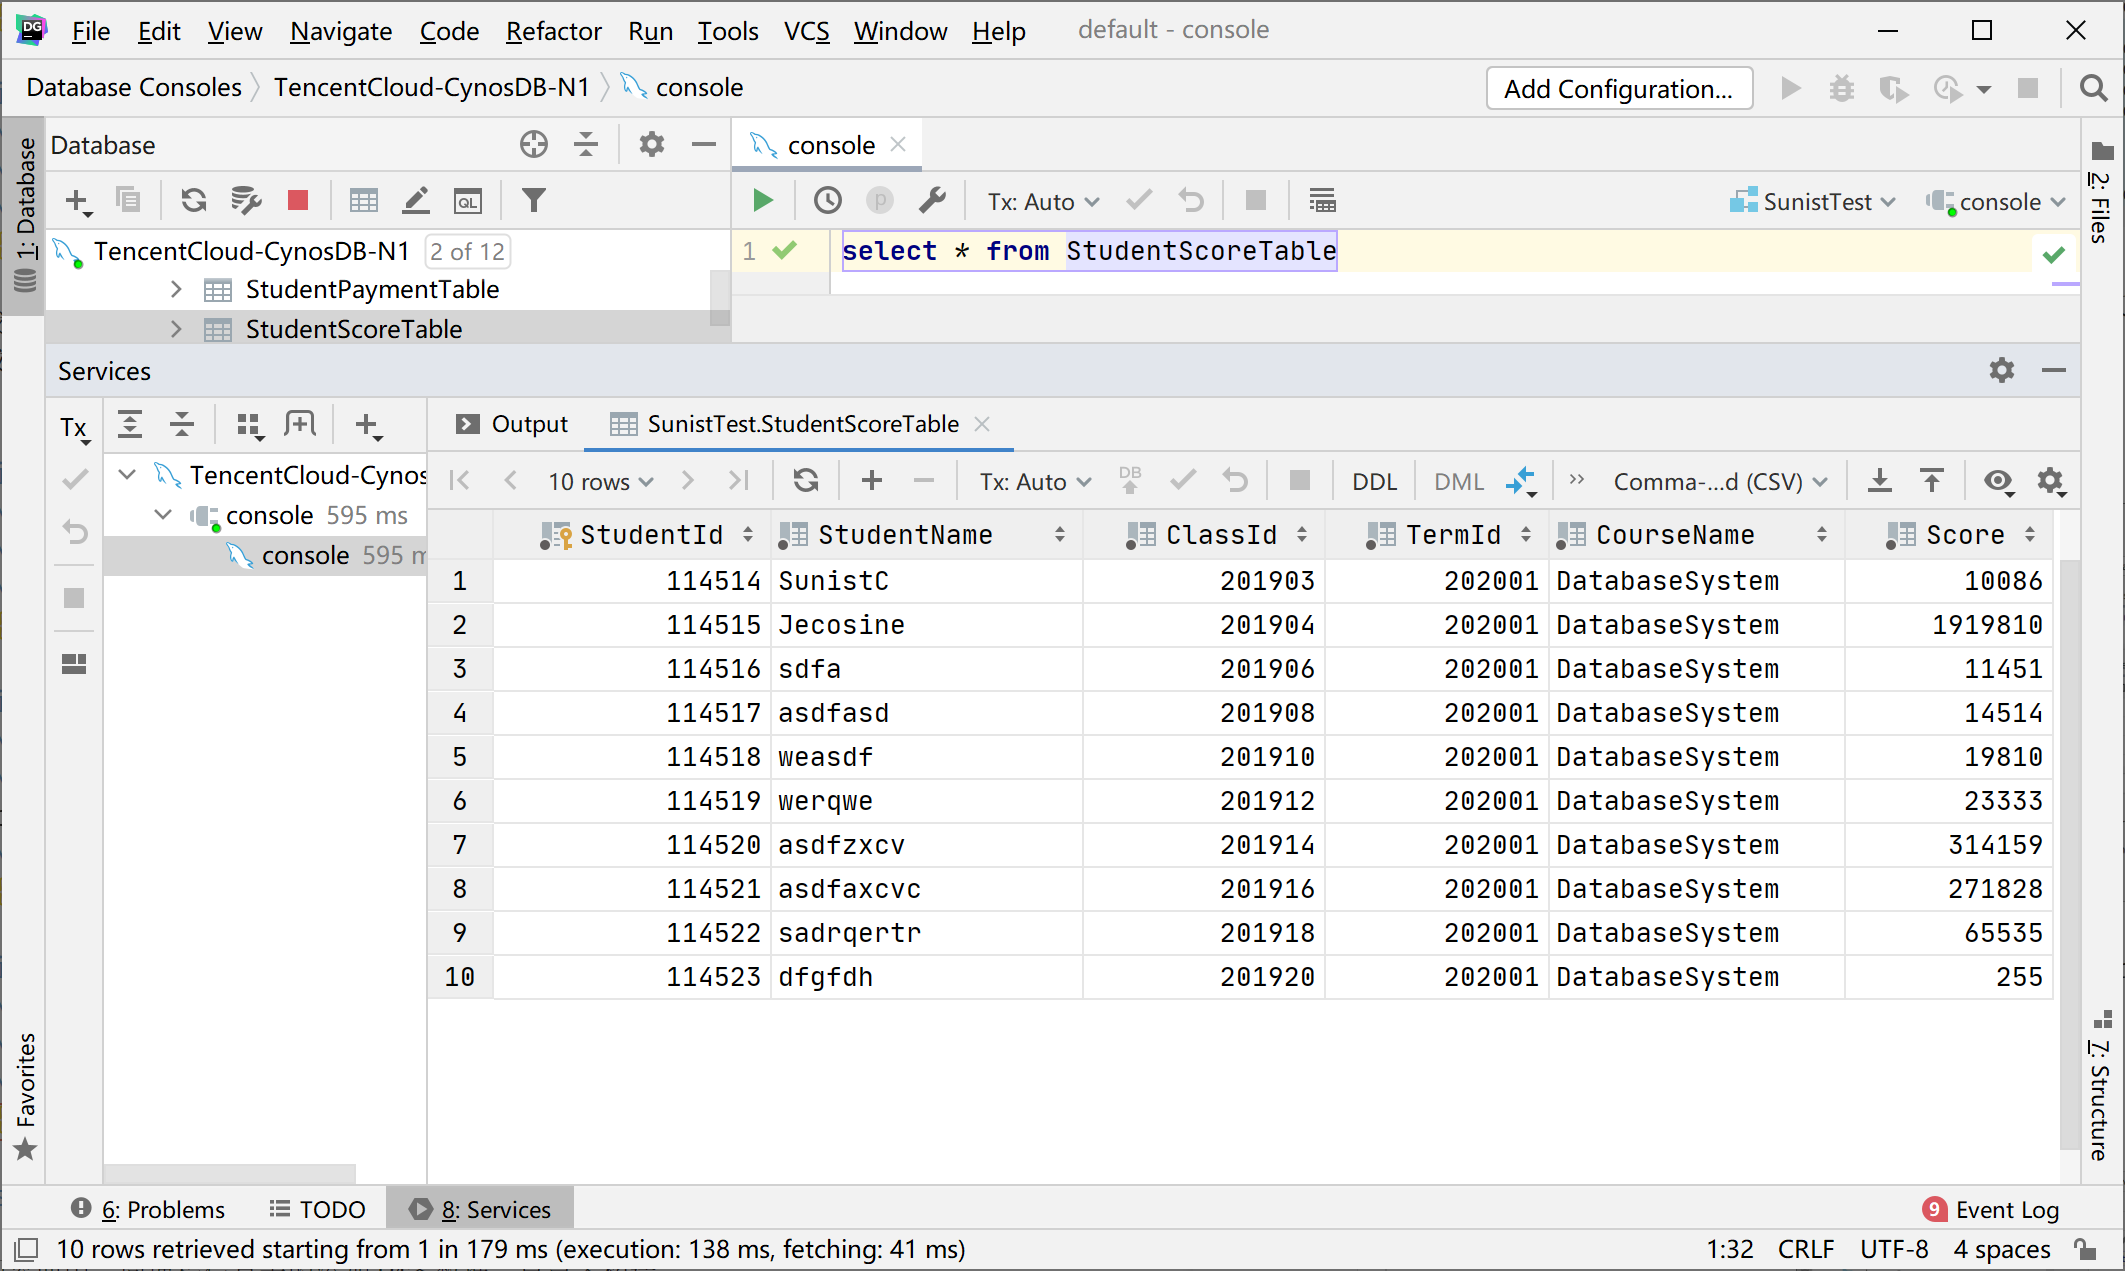
\includegraphics[width=15cm]{../Images/StudentScoreTable_OnImported.png}
    \caption{导入完成的学生成绩信息表}
\end{figure}

\newpage

\subsubsection{视图方式添加数据}

在视图界面中,向课程信息表的添加10条数据,自己各构造。

我们构造了十条课程信息表的数据在DataGrip的视图界面内,如下图7所示。

\begin{figure}[htbp]
    \centering
    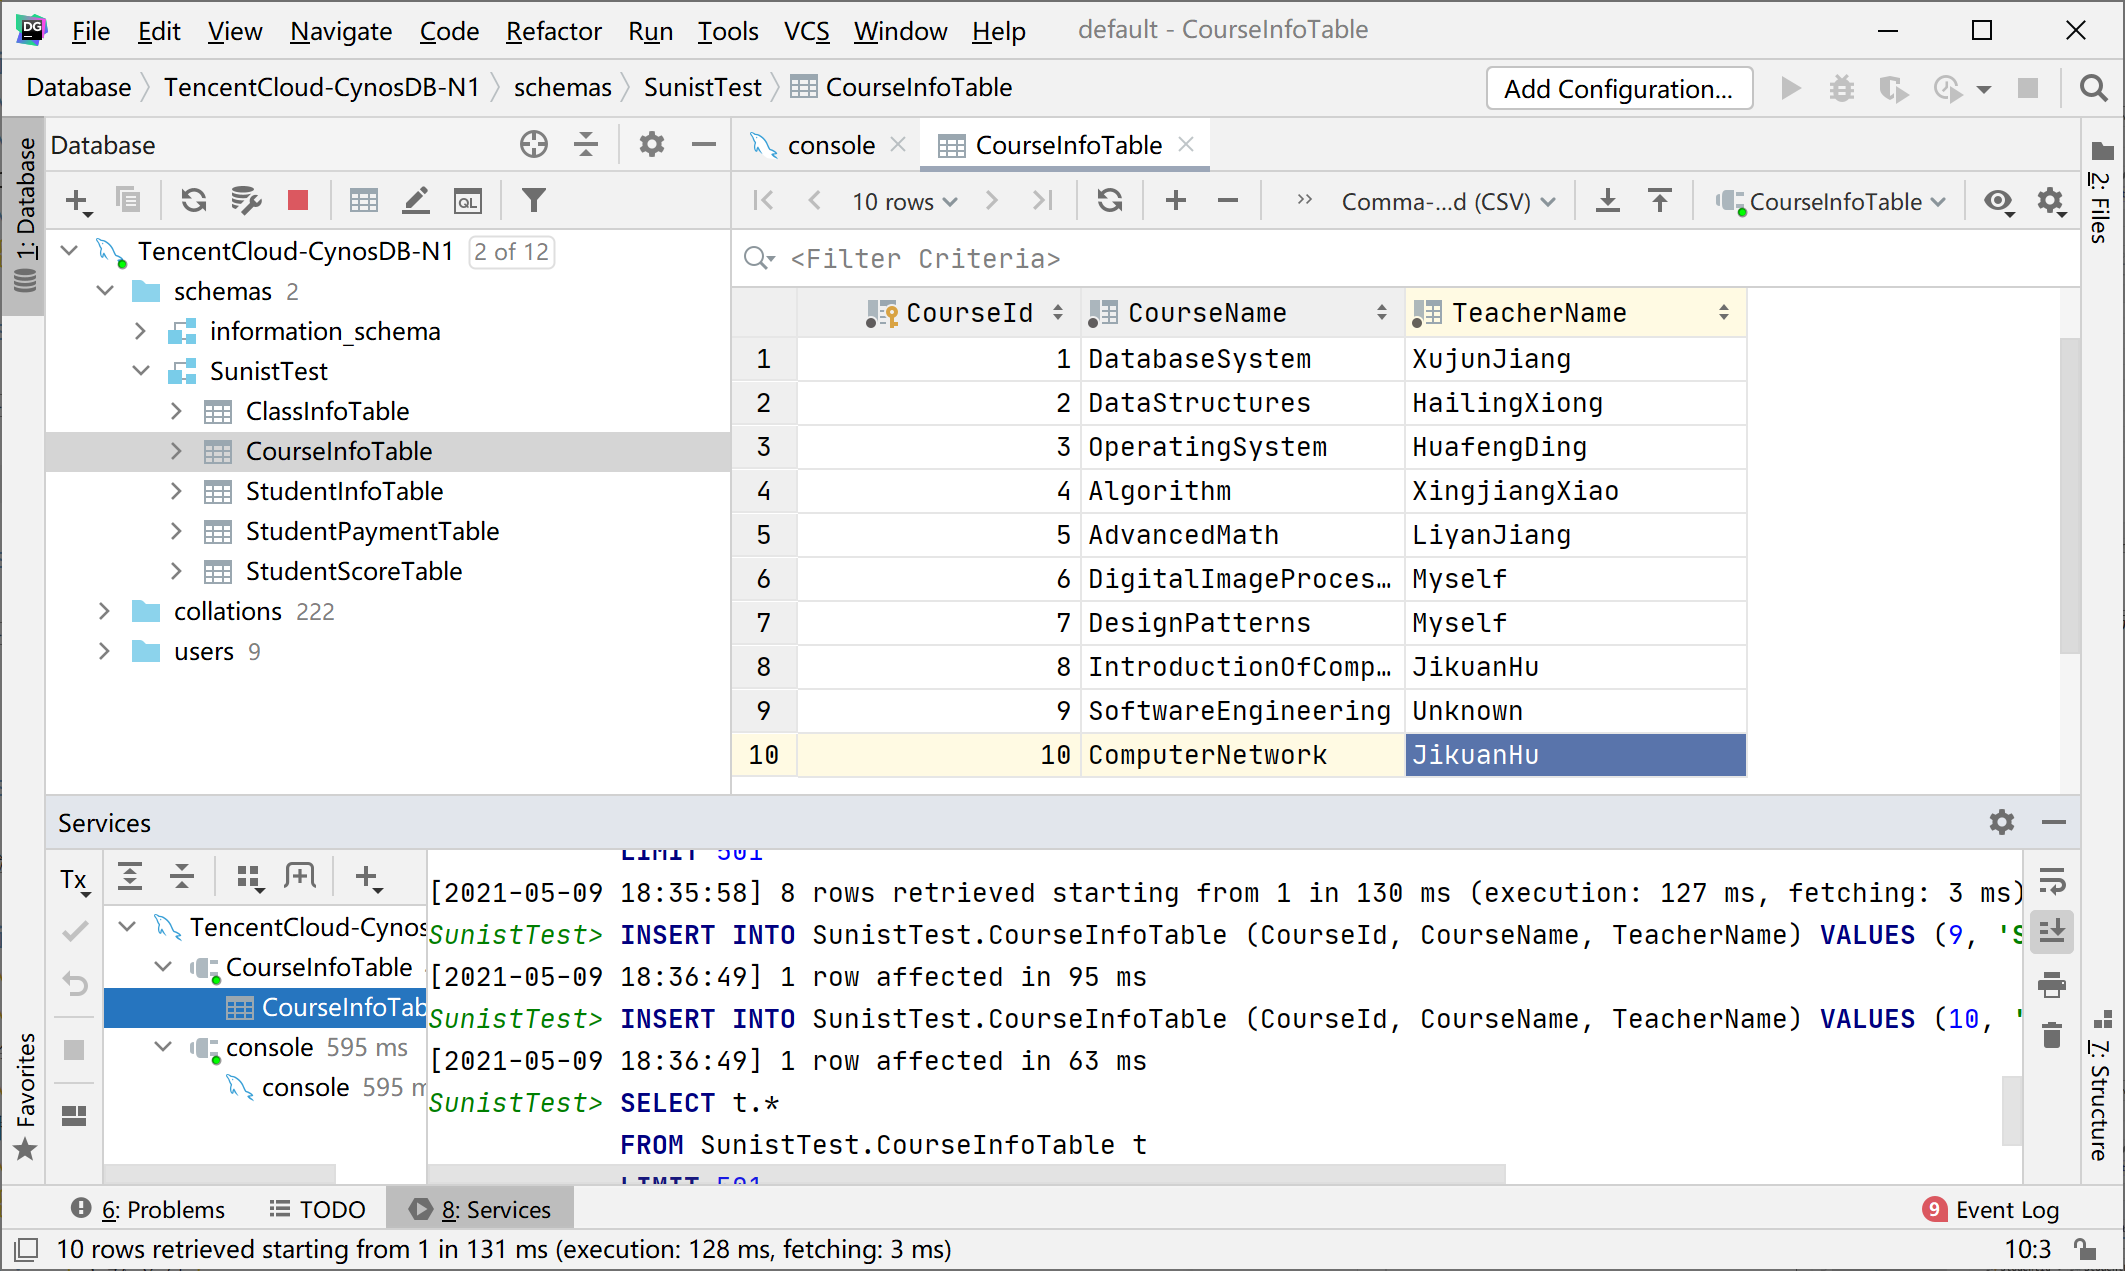
\includegraphics[width=14cm]{../Images/CourseInfoTable_OnImport.png}
    \caption{构造的课程信息表}
\end{figure}

然后我们执行添加指令(Ctrl+Enter),结果如下图8所示。

\begin{figure}[htbp]
    \centering
    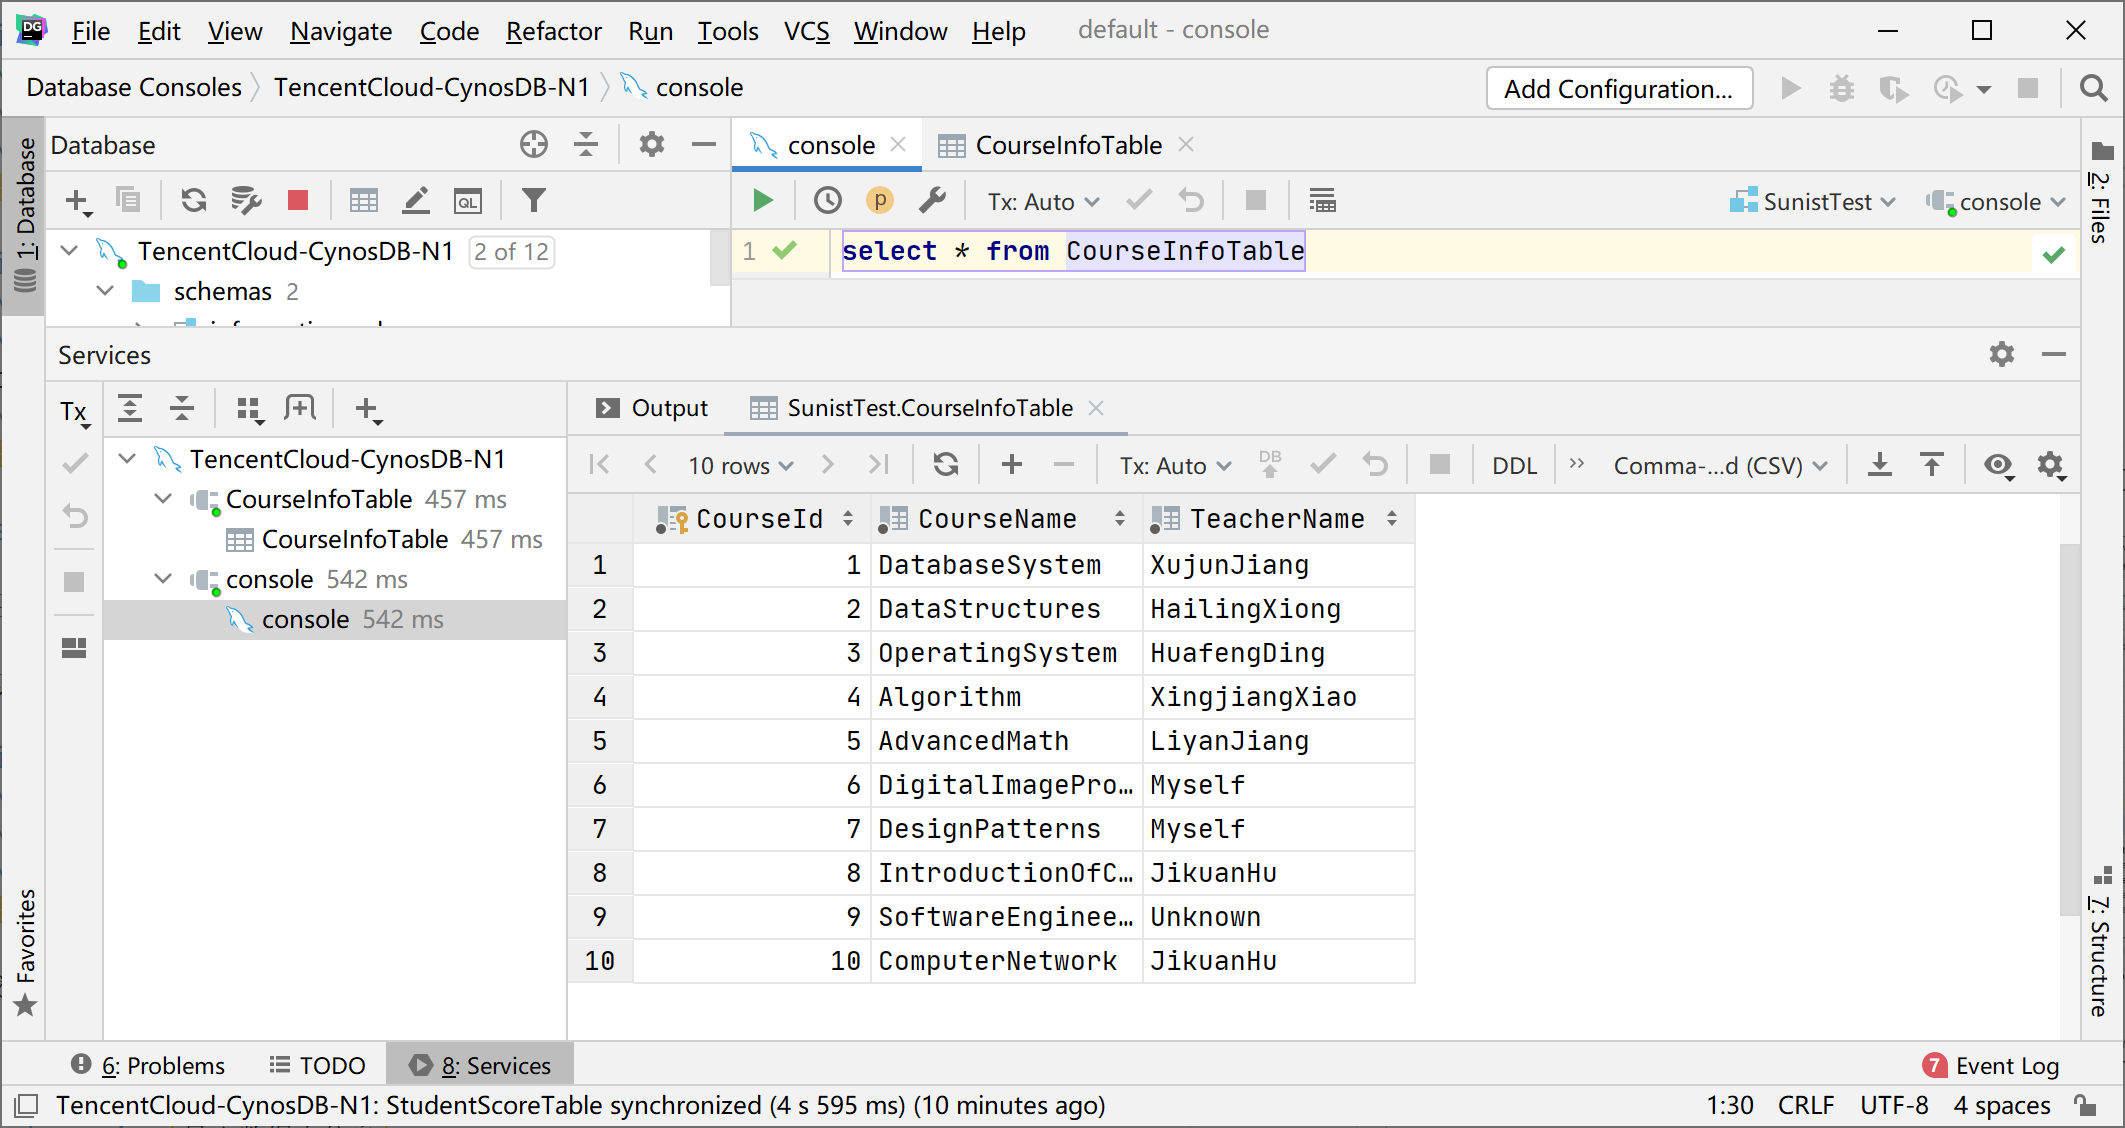
\includegraphics[width=14cm]{../Images/CourseInfoTable_OnImported.png}
    \caption{导入完成的课程信息表}
\end{figure}

\newpage

\subsubsection{导出数据表信息}

在视图界面中,导出数据表信息,包含Excel格式和TXT文件格式。

我们在DataGrip中进行导出操作,过程如下图9所示,由于TSV,CSV,XLSX格式差别只有导出格式,此处省略了其余格式步骤。

\begin{figure}[htbp]
    \centering
    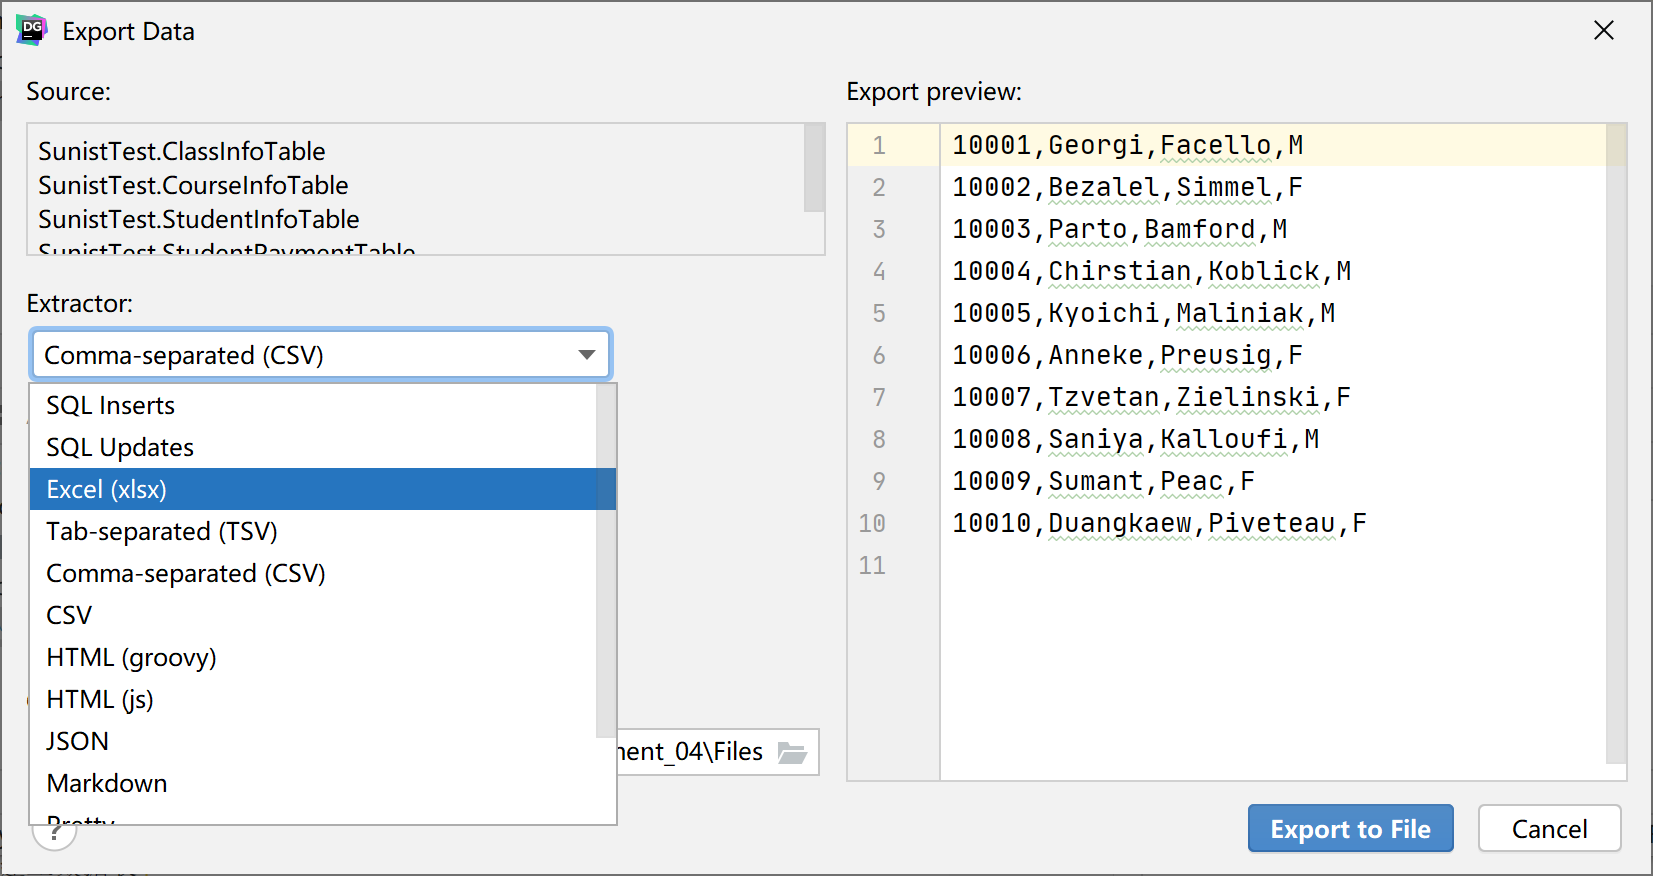
\includegraphics[width=15cm]{../Images/Database_OnExport.png}
    \caption{导出数据库}
\end{figure}

导出完毕的数据库(此处列举三张表)如下:

\begin{enumerate}
    \item CommaSeparatedVersion(CSV格式)
    \item TabSeparatedVersion(TSV格式)
    \item Excel工作表(XLSX格式)
\end{enumerate}

其中,CSV格式使用逗号分隔,导出的是班级信息表;TSV格式使用的是制表符分隔,导出的是班级信息表;XLSX是Excel工作表格式,导出的是学生成绩信息表。

其中CSV能被作者的Visual Studio Code插件读取,所以显示为表格而不是文本文件。

三张表格如下图10 - 12所示:

\begin{figure}[htbp]
    \centering
    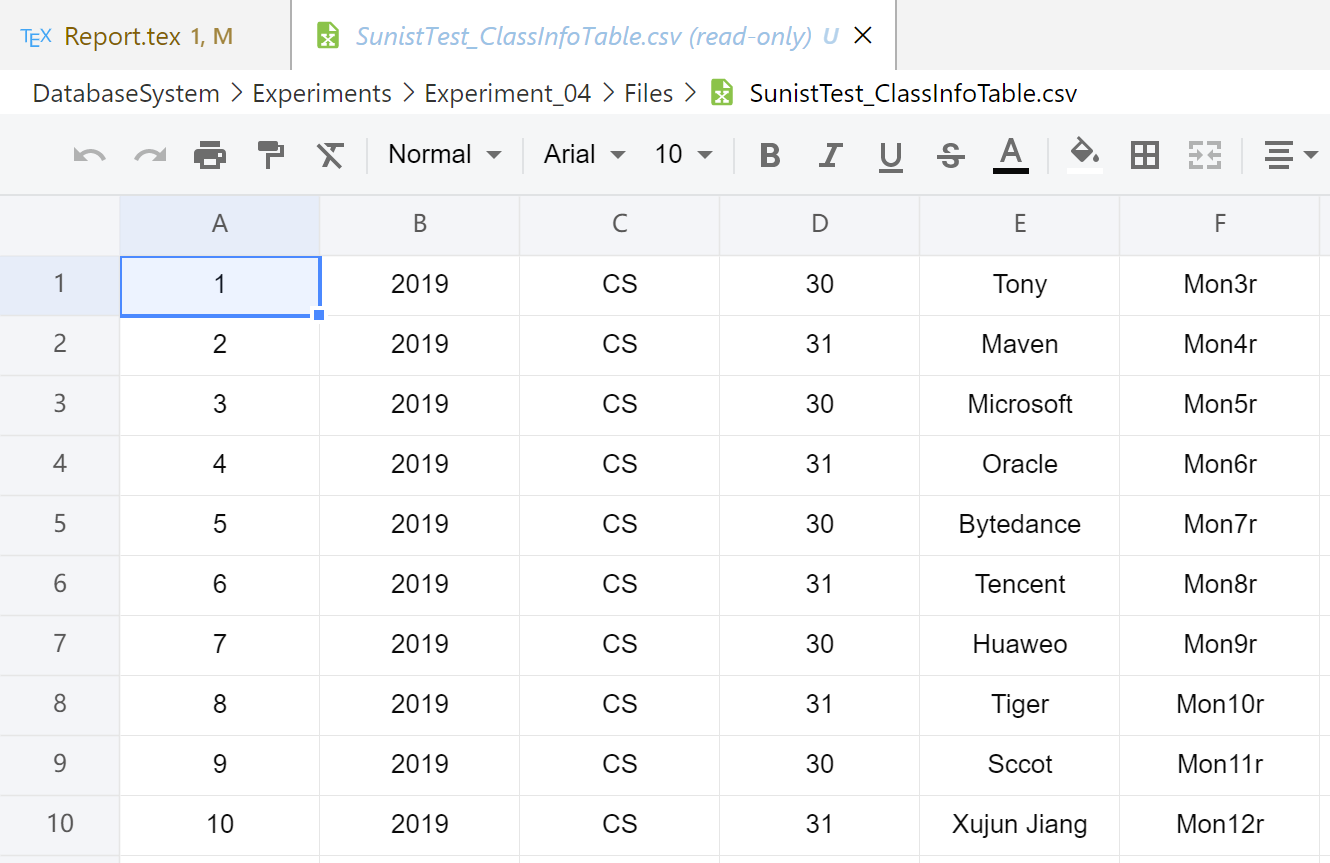
\includegraphics[width=10cm]{../Images/Database_OnExported_CSV.png}
    \caption{导出完毕的CSV格式数据}
\end{figure}

\begin{figure}[htbp]
    \centering
    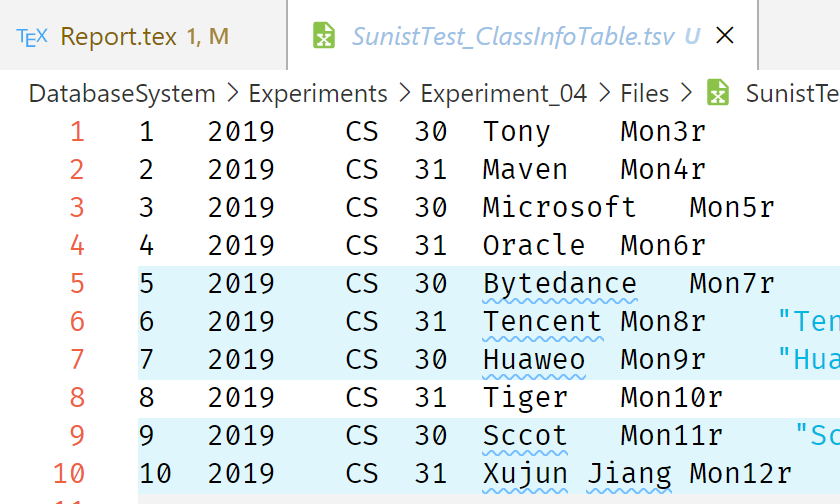
\includegraphics[width=10cm]{../Images/Database_OnExported_TSV.png}
    \caption{导出完毕的TSV格式数据}
\end{figure}

\begin{figure}[htbp]
    \centering
    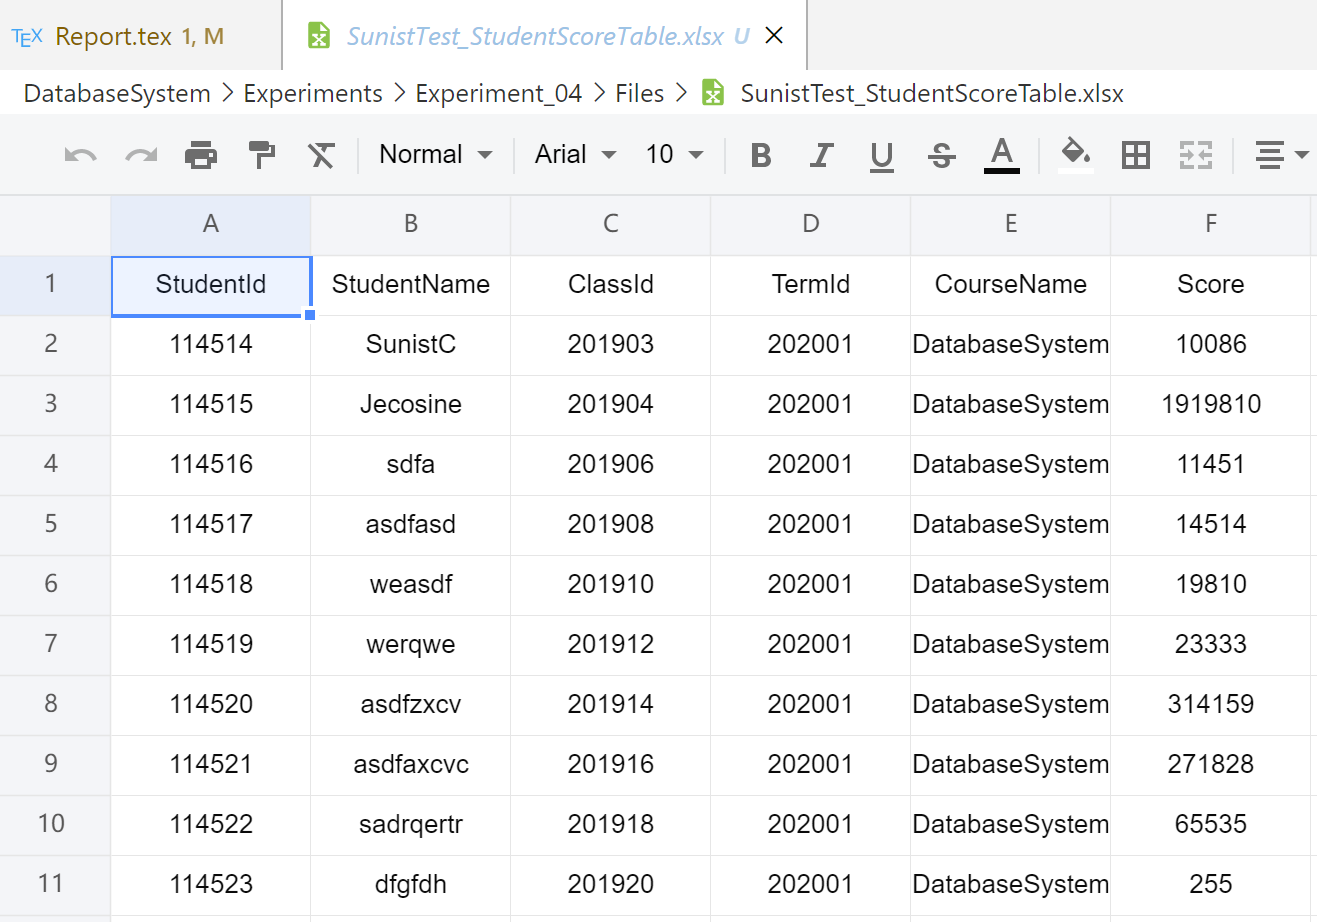
\includegraphics[width=10cm]{../Images/Database_OnExported_XLSX.png}
    \caption{导出完毕的XLSX格式数据}
\end{figure}

\newpage

\subsection{命令方式建立数据表}

向实验三教材第三章的例子用到的三张表添加数据\footnote{此处作者使用了DataGrip的控制台与MysqlClient结合进行命令操作}。

\subsubsection{使用Insert命令添加数据}

用Insert命令向表(Course)中插入书上教材第三章例子中的数据。

输入的指令如下图13所示。

\begin{figure}[htbp]
    \centering
    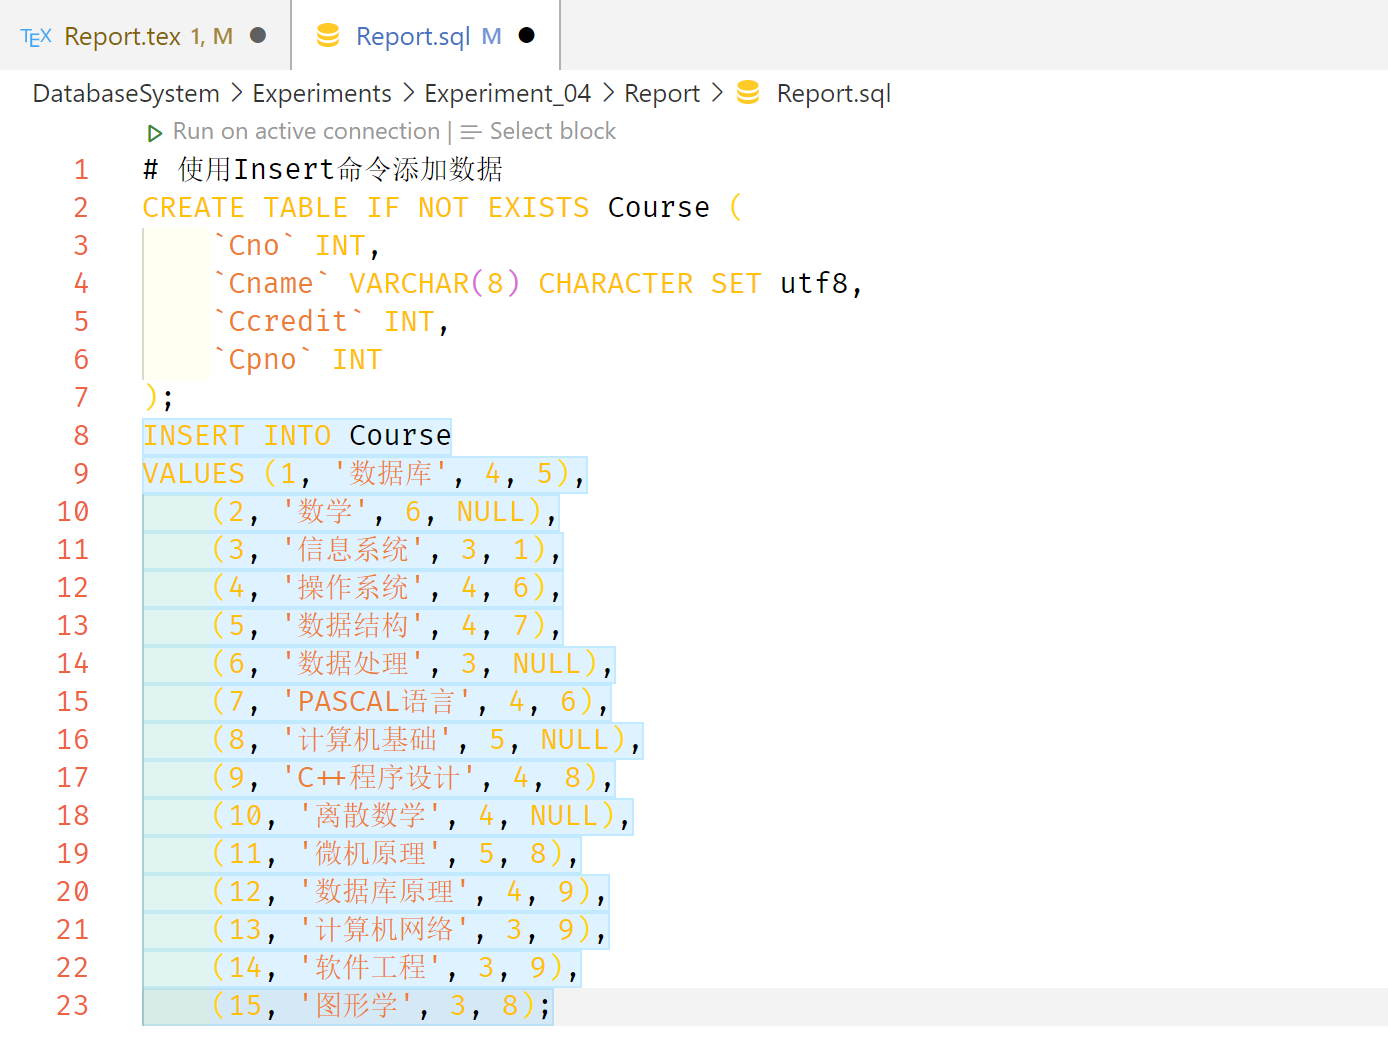
\includegraphics[width=15cm]{../Images/InsertCommand_OnImport.png}
    \caption{使用Insert命令添加数据的指令}
\end{figure}

\subsubsection{使用命令导入Excel工作表中的数据}

此处我们在查询了Stackoverflow,CSDN,GitHub,Microsoft论坛,Oracle论坛后,未发现MySQL能够直接导入xls/xlsx格式的数据\footnote{不能导入的原因在总结处},必须使用中间件、第三方库或对MySQL进行二次开发等方式才能够导入xls/xlsx格式的数据,此处我们将其保存为csv格式的数据,进行导入。

\newpage

我们先将实验给定的xls格式Student表导出为csv表格。导出结果如下图14所示。

\begin{figure}[htbp]
    \centering
    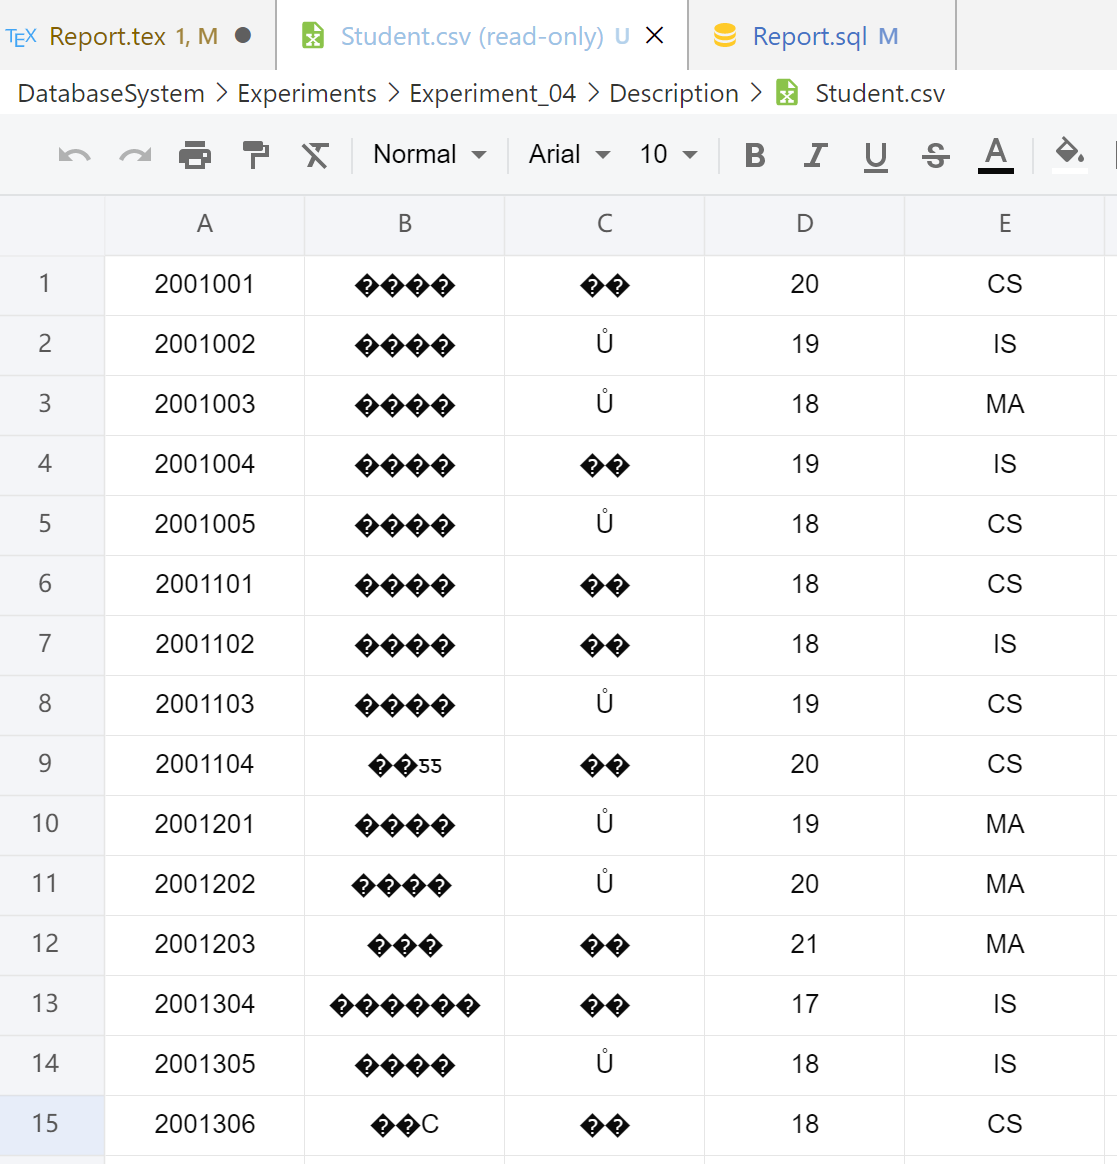
\includegraphics[width=15cm]{../Images/ImportWithCommand_OnImport.png}
    \caption{导出Student为CSV格式}
\end{figure}

为什么会出现乱码呢?是实验给定的表格中文字符集使用的是GBK编码(Windows Notepad的编码方式),而作者的预览器使用的是与MySQL一致的UTF-8格式,两者并不兼容导致的。

在作者经过一晚上四个小时的探索后,发现本实验要求的使用命令"LOAD DATA LOCAL INFILE \{\$filename\} INTO TABLE \{\$tablename\}"导入数据时,DataGrip所要求MySQL最低版本为\footnote{此处作者使用的MySQL版本为5.7.12(腾讯云分布式数据库定制版)}8,错误信息如下图15所示,所以作者只能使用MysqlClient登录进行操作。

\begin{figure}[htbp]
    \centering
    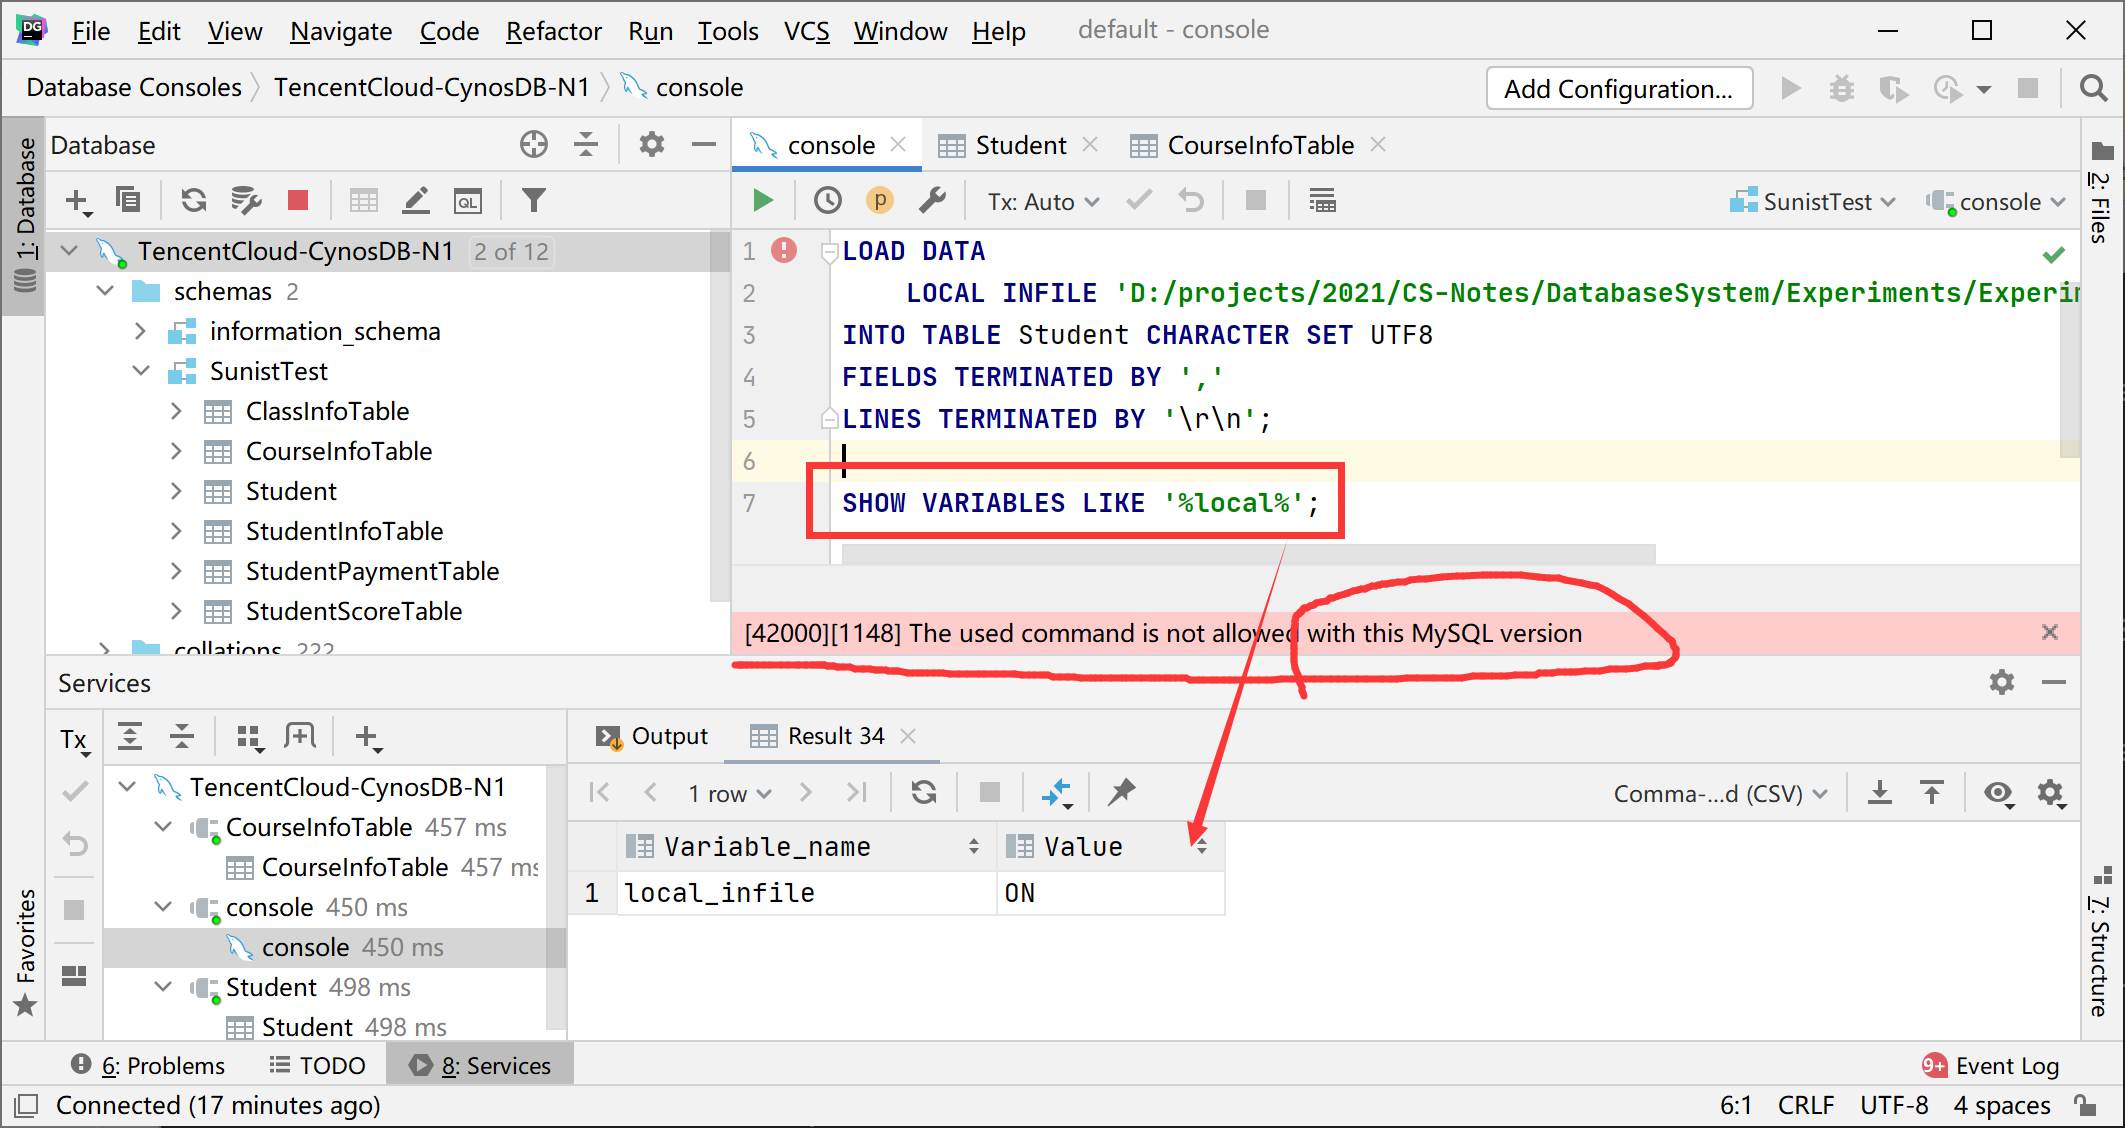
\includegraphics[width=12cm]{../Images/ImportWithCommand_ErrorOnDataGrip.png}
    \caption{DataGrip不允许此版本的MySQL使用LOAD DATA INFILE指令}
\end{figure}

由于csv数据使用的字符编码是GBK,而数据库的编码为UTF8,所以导入会出错,如下图16所示,我们改用GBK作为字符编码导入,如下图16所示。

\begin{figure}[htbp]
    \centering
    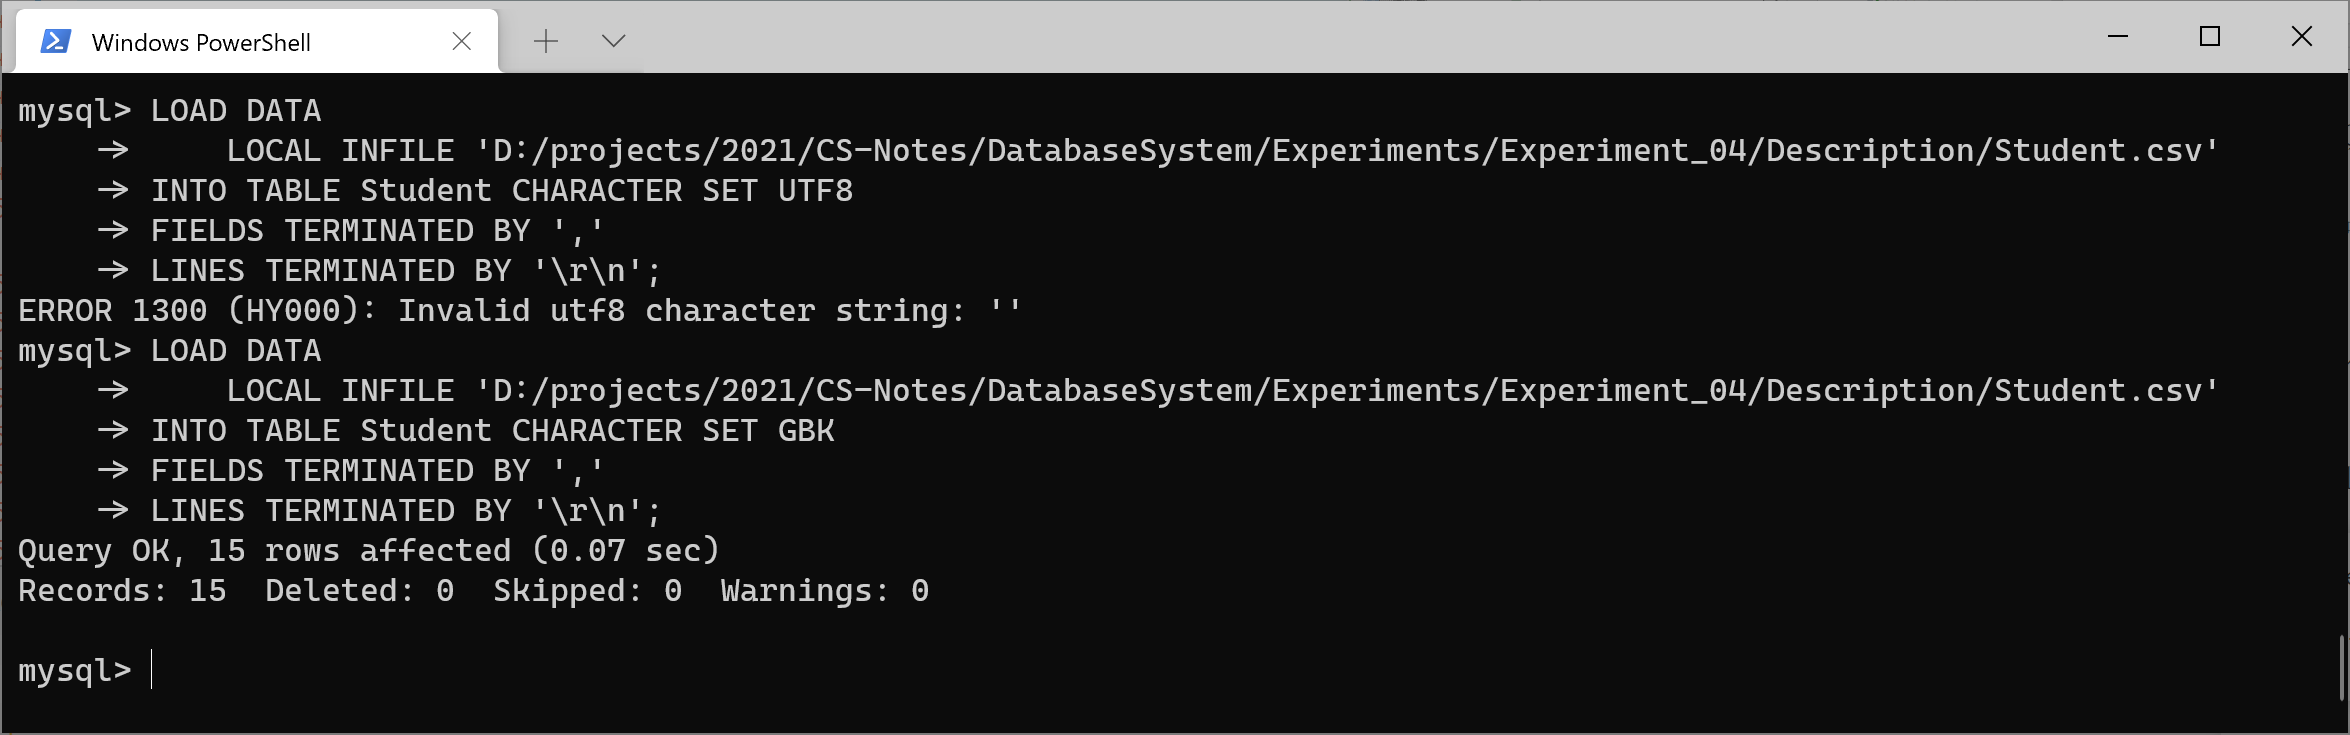
\includegraphics[width=15cm]{../Images/ImportWithCommand_OnLoad.png}
    \caption{使用MysqlClient进行导入操作}
\end{figure}

导出后的结果如下图17所示,因为作者先前强制使用UTF8导入了GBK编码的字符,所以前15条记录是乱码记录。

\begin{figure}[htbp]
    \centering
    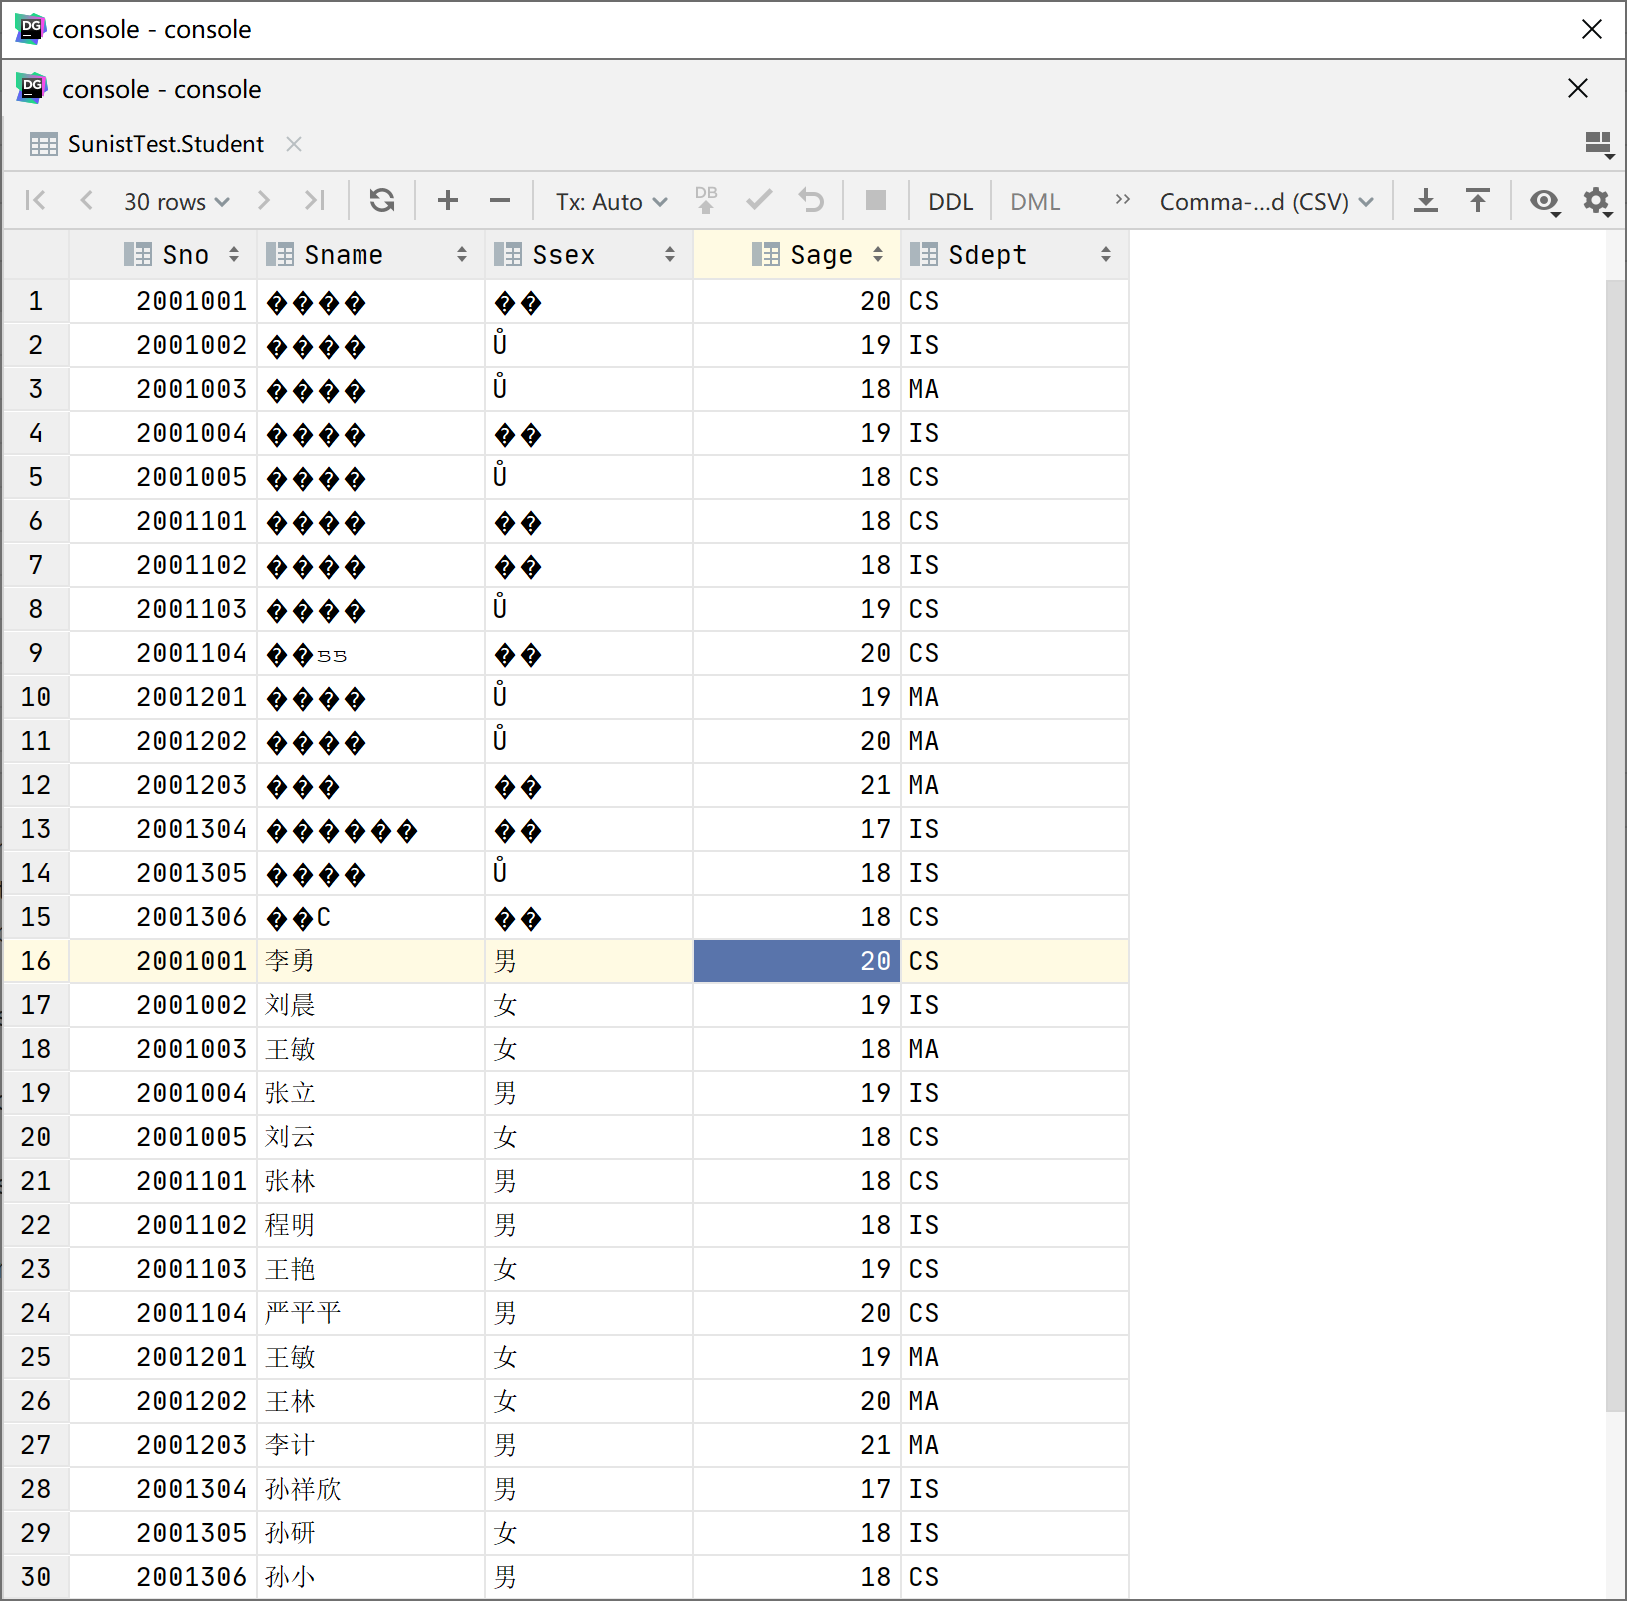
\includegraphics[height=10cm]{../Images/ImportWithCommand_OnLoaded.png}
    \caption{导入完成的结果}
\end{figure}

\subsection{使用命令导入txt格式的数据}

由于csv格式其实就是txt格式,上节已进行过,本节略。

\subsection{使用命令导出数据表}

我们使用SELECT INTO OUTFILE指令进行导出,其指令如下图18所示。

\begin{figure}[htbp]
    \centering
    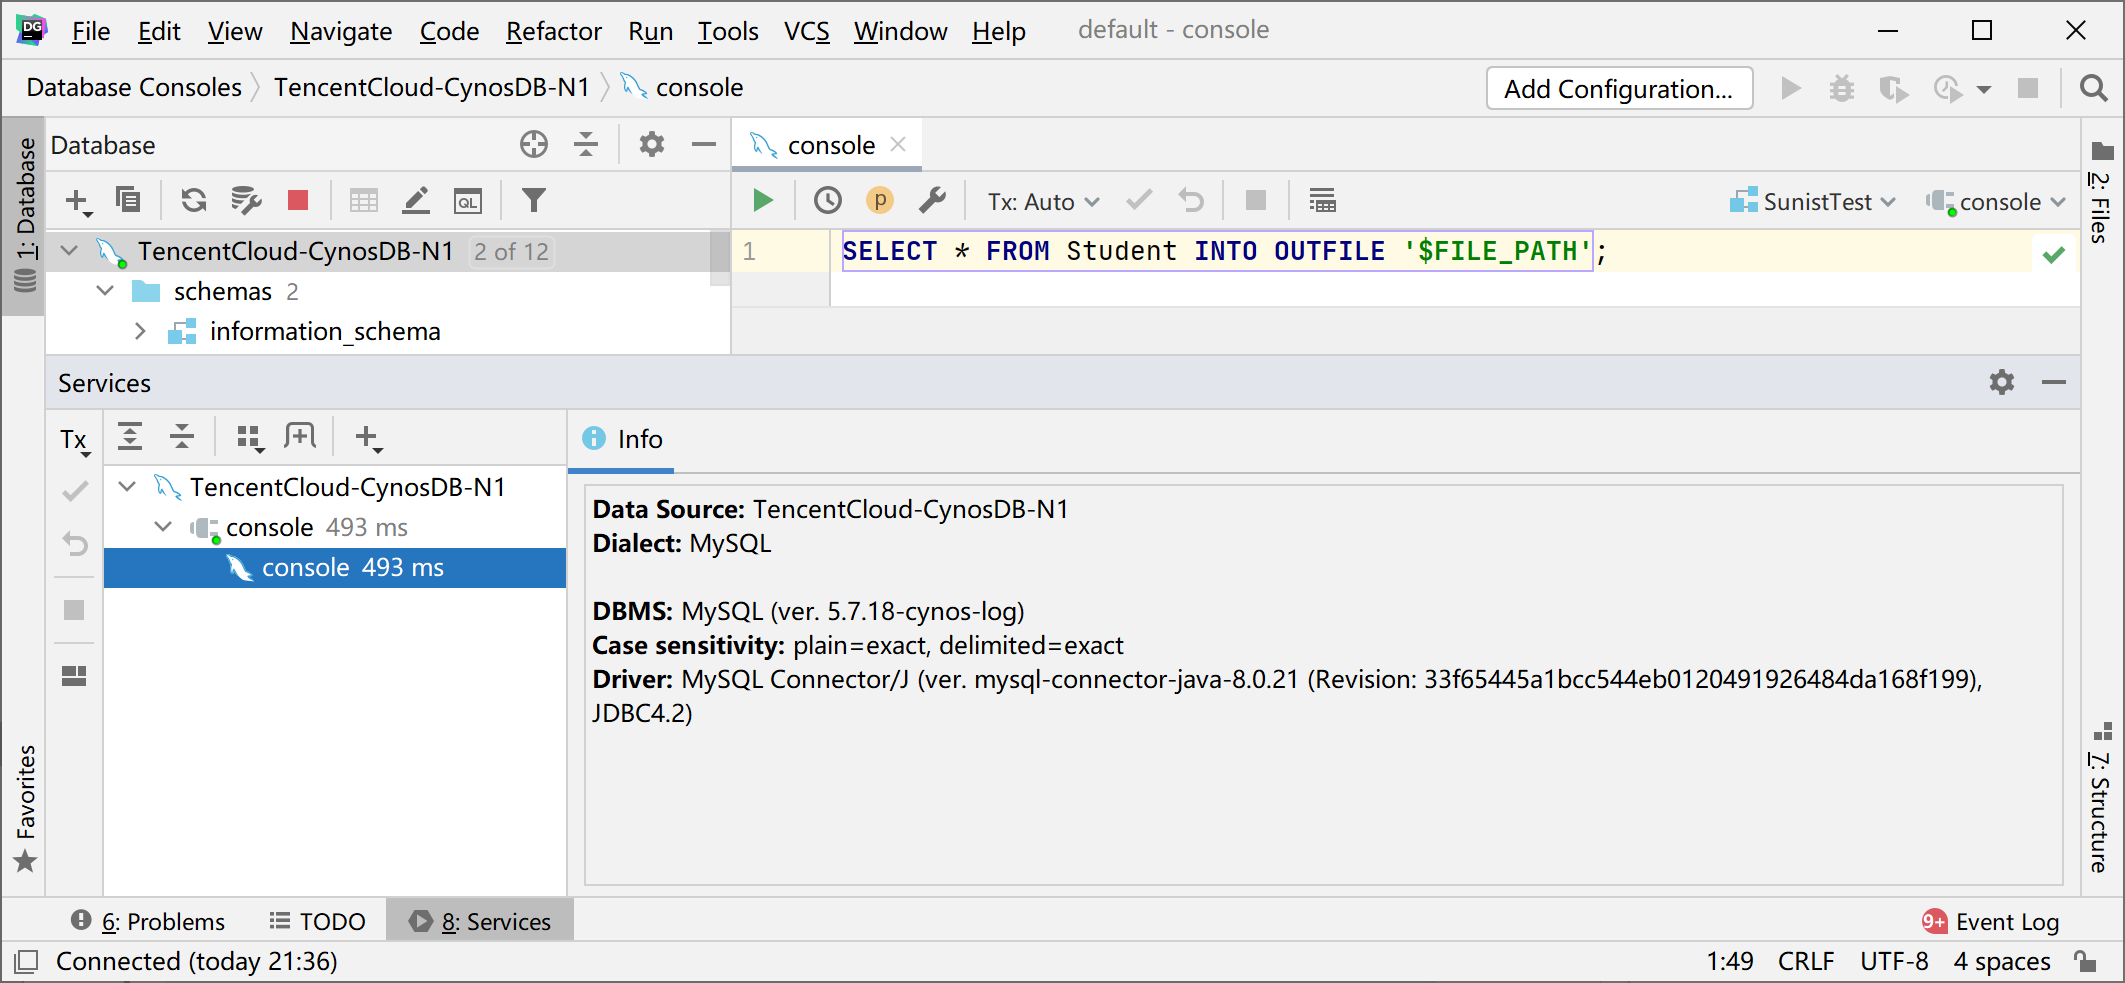
\includegraphics[width=15cm]{../Images/ExportWithCommand.png}
    \caption{使用Select Into Outfile导出的过程}
\end{figure}

但由于此处使用的是远程服务器,作者没有读取服务器文件的权限\footnote{此处作者只能使用Mysql的端口与Mysql进行通信,而无法通过Mysql读取其导出的文件,当然远程服务器也没有给予Mysql可以导出文件的权限},所以此处作者只能使用mysqldump进行导出,导出的文件为.sql文件,如下图19所示。

\begin{figure}[htbp]
    \centering
    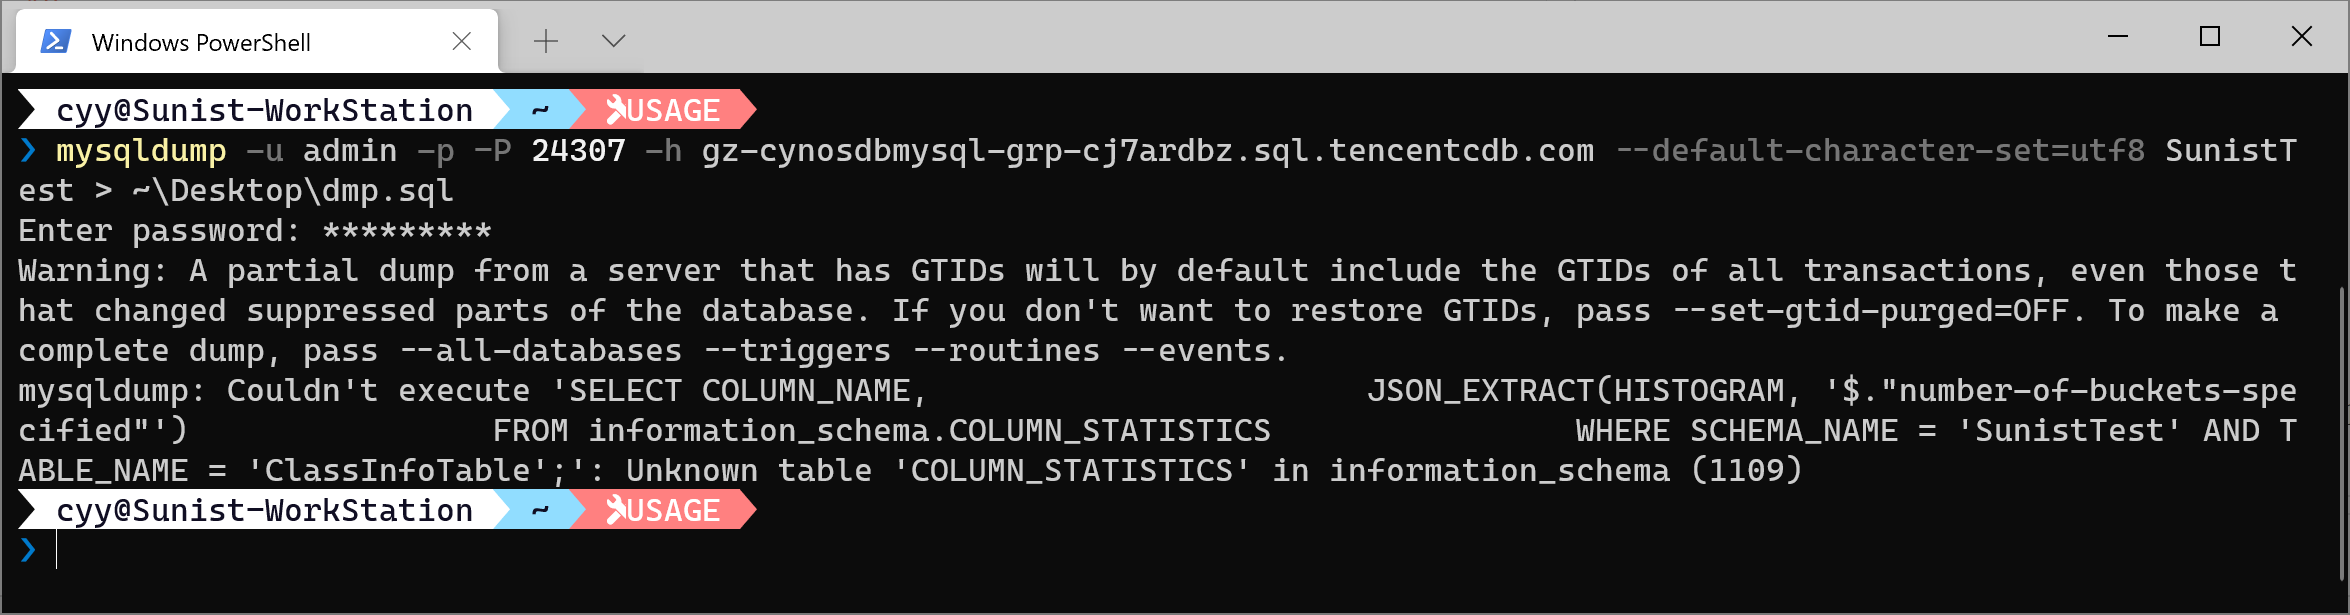
\includegraphics[width=15cm]{../Images/ExportWithCommand_OnExported.png}
    \caption{使用MysqlDump导出的过程}
\end{figure}

导出结果如下图20所示(此处导出的是表结构),在本地数据库重新建表,执行普通导出操作即可\footnote{此处作者本地未安装有Mysql-Server,故无法进行此实验}。

\begin{figure}[htbp]
    \centering
    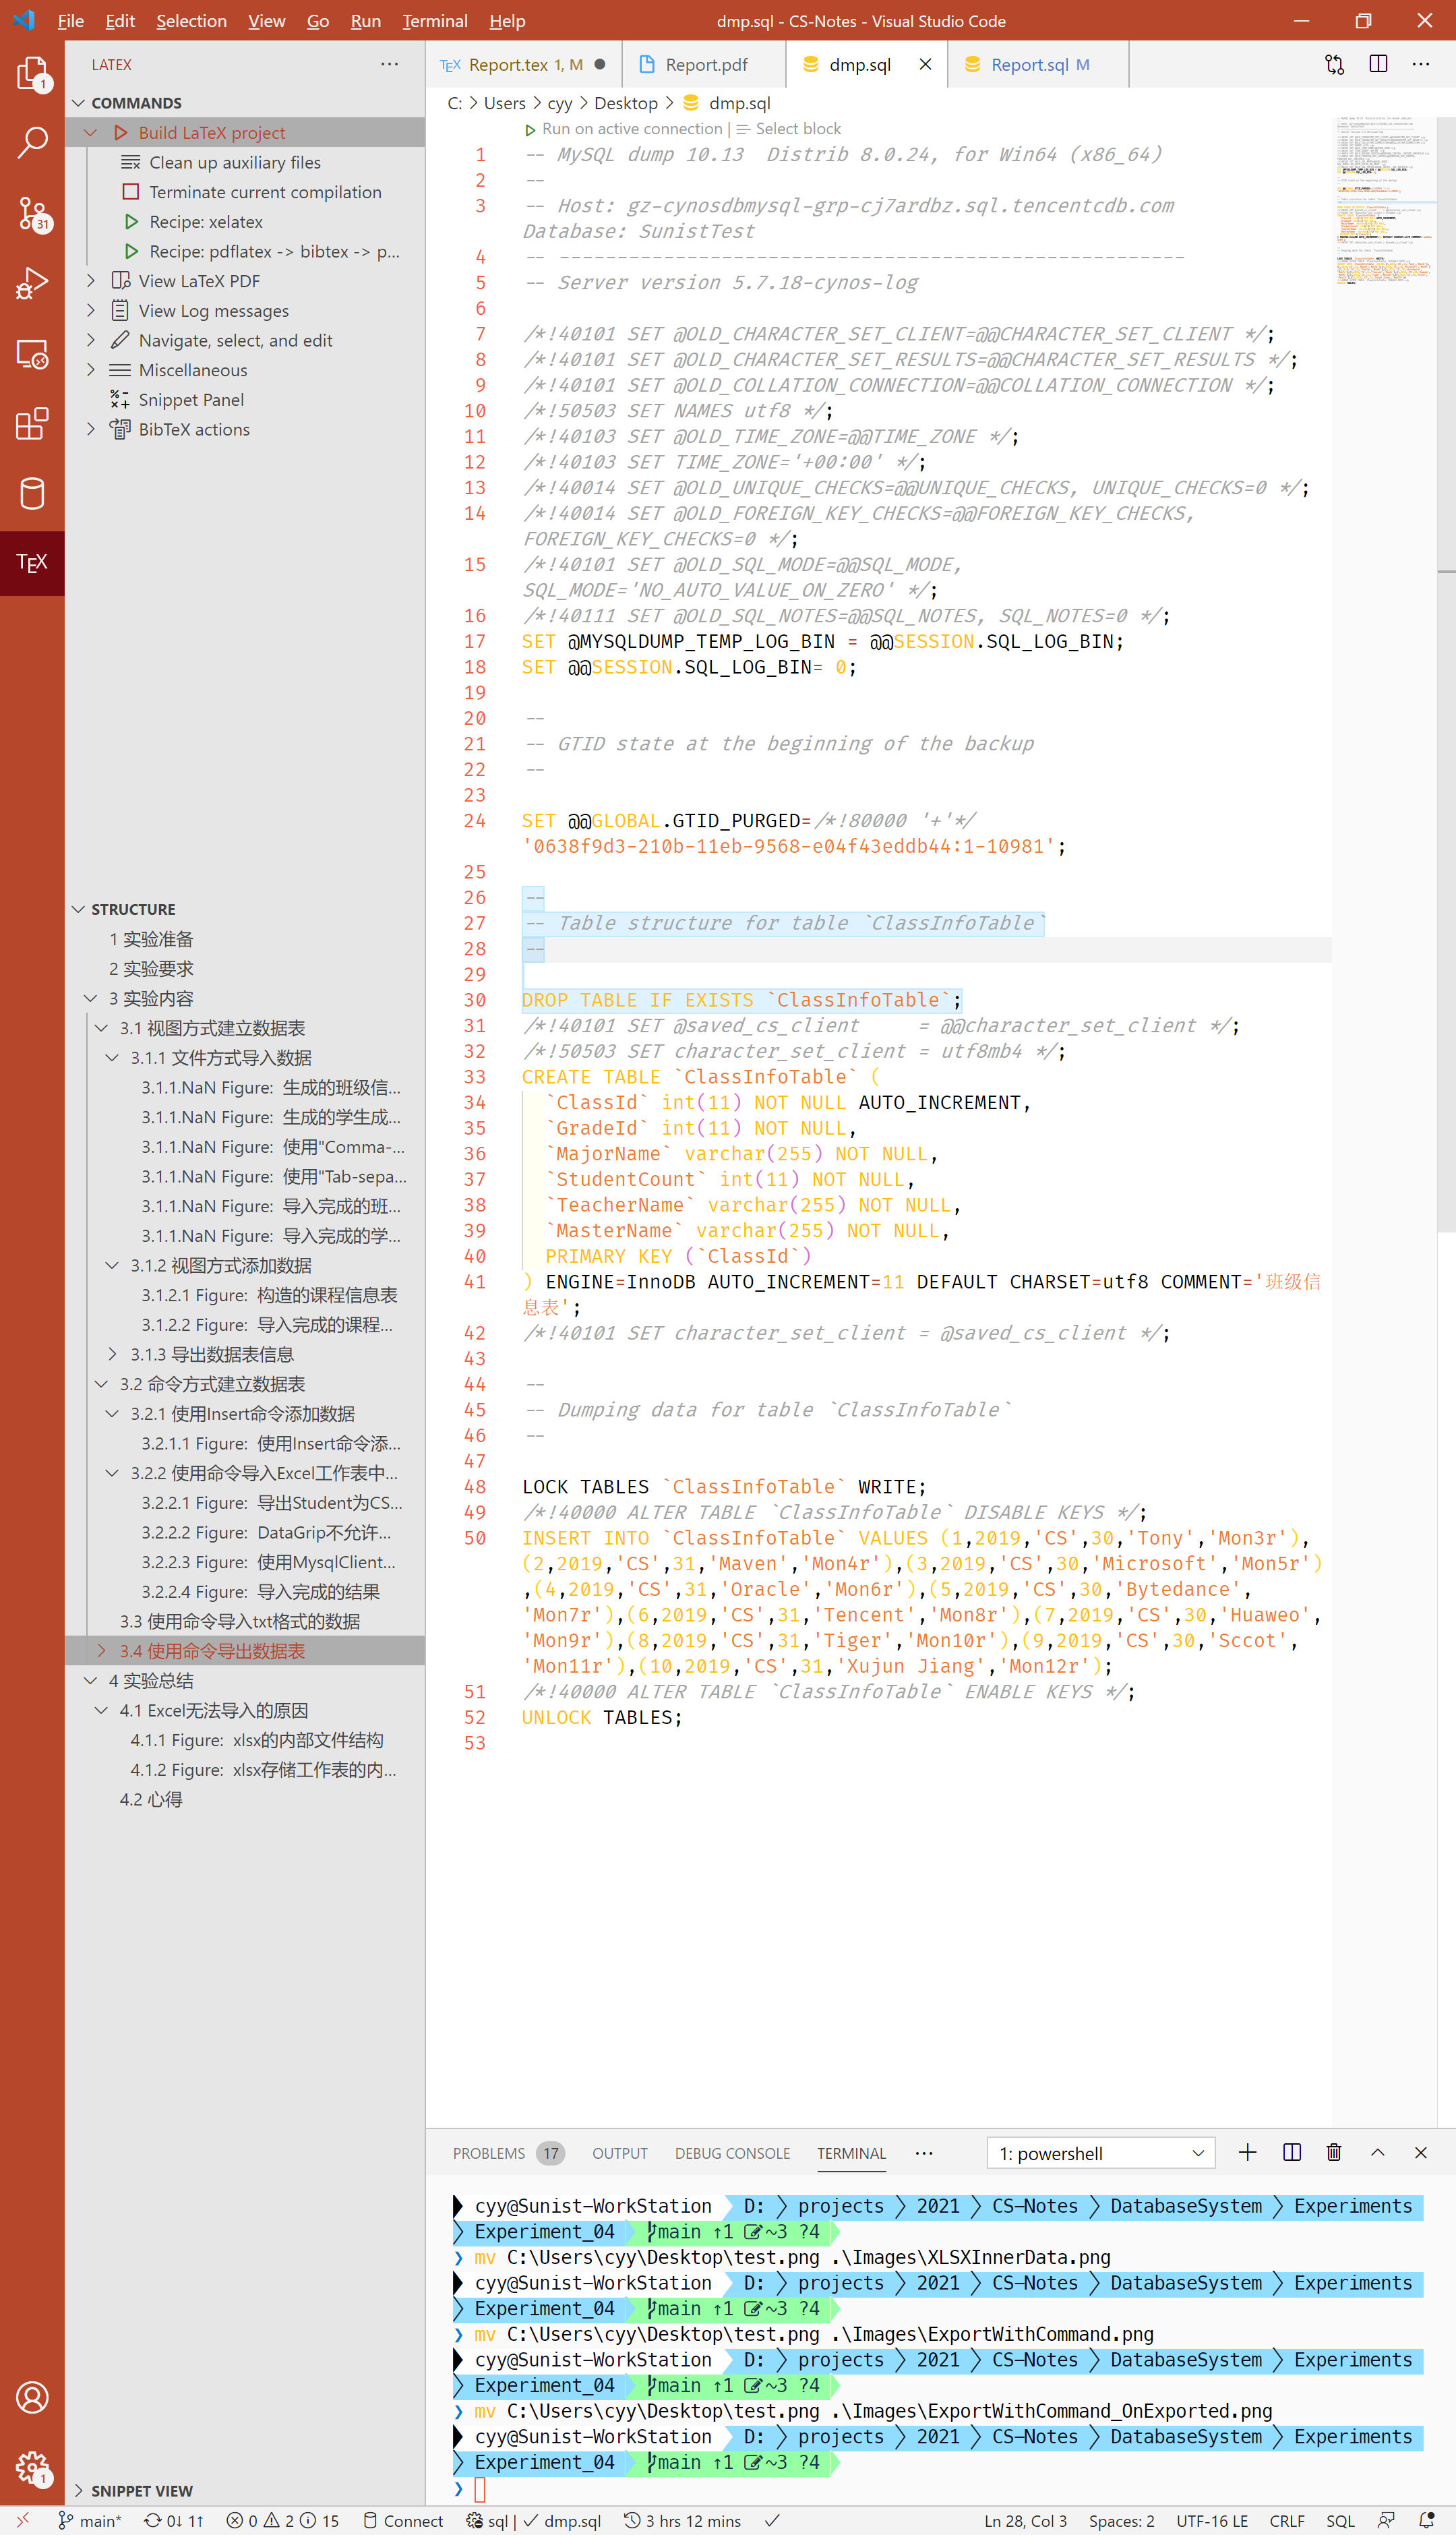
\includegraphics[height=25cm]{../Images/ExportWithCommand_ExportFile.png}
    \caption{使用MysqlDump导出的结果}
\end{figure}

\newpage

\section{实验总结}

\subsection{Excel无法导入的原因}

因为MySQL的load data infile是通过字符流的方式进行读写操作的。而Excel内部的结构根本不是文件,而是一个xml文件作为工作簿的信息,加上三个文件夹\_rels,xl和docProps存储数据信息的,其中工作表信息存储在xl文件夹中,内部真实结构是xml标记文档,虽然其本质依旧是文本文件,但是其信息已经被复杂的文件层级结构加上Office的标记给层层覆盖,使得MySQL无法直接进行读取。读取此类文件,需要先将xlsx文件解压缩,再提取其表格数据文件,剥离Office冗余标记后才能进行读取,而MySQL的load data infile指令根本无法进行此类复杂工作,必须借助第三方工具。其中,xlsx的层级结构如下图21所示,数据表的数据信息如下图22所示。

\begin{figure}[htbp]
    \centering
    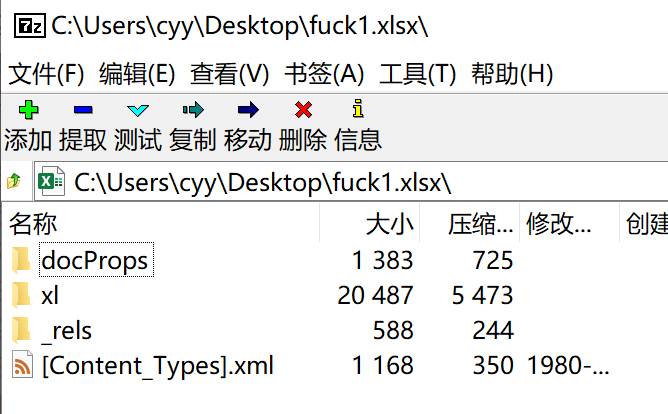
\includegraphics[height=5cm]{../Images/XLSXStructures.png}
    \caption{xlsx的内部文件结构}
\end{figure}

\begin{figure}[htbp]
    \centering
    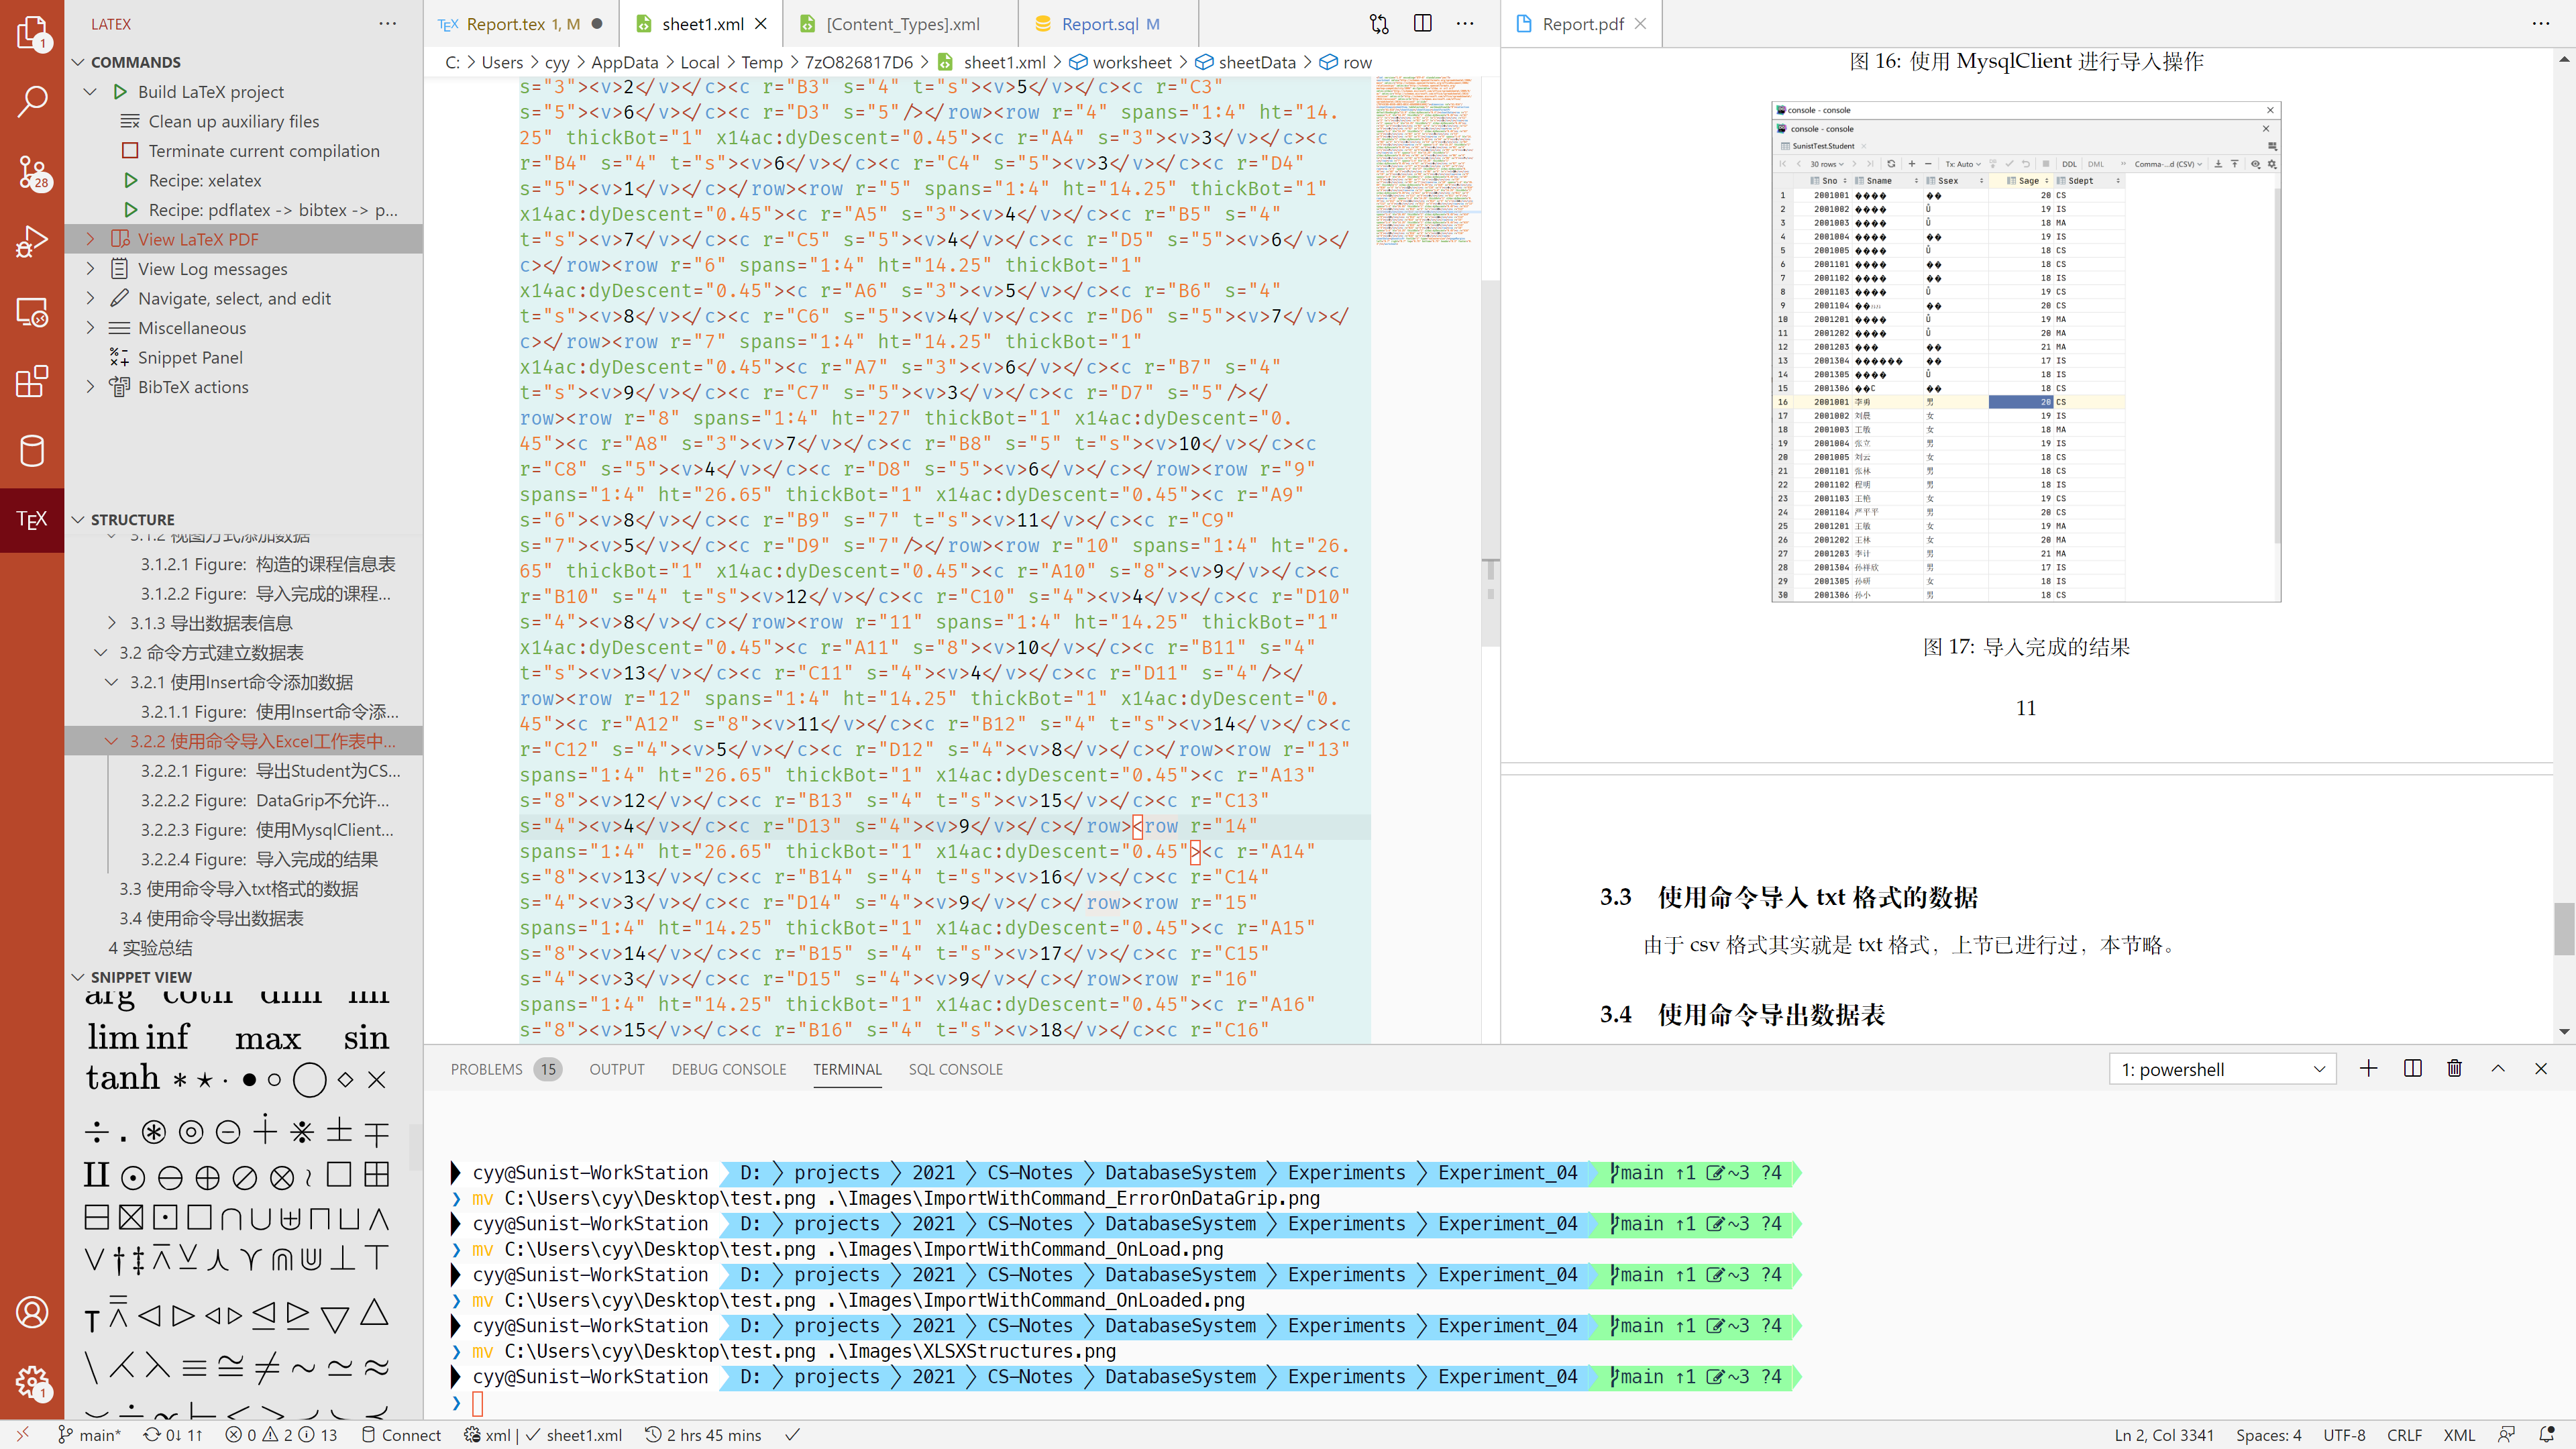
\includegraphics[width=15cm]{../Images/XLSXInnerData.png}
    \caption{xlsx存储工作表的内部数据}
\end{figure}

\subsection{心得}

\begin{enumerate}
    \item 设计数据表时一定要注意字符集,此项一定要与产生数据的后端、前端沟通好,避免因为字符集的问题出错。目前互联网普遍使用的字符集为utf8mb4,此字符集不仅能存储所有的常见字,也能存储诸如emoji表情一类的拓展文字,但所使用的数据库驱动引擎必须为InnoDB。
    \item 要善于从Stackoverflow,GitHub等论坛寻找解决问题的方法,如此次实验设置了无法完成的操作,不经过深入探讨根本无法得知出错的原因。
    \item 使用DataGrip,WorkBench,Navicat等图形化数据库管理系统时,需要先了解其支持指令、所需数据库版本等信息,此次实验出现的'used command is not allow with this MySQL Version'等问题是应该要事前知道并寻找替代解决方案的。
    \item \LaTeX 的字体在macOS与Windows并不一样,如在mac/Linux上显示为'FiraCode NF'的等宽字体在Windows上显示为'FiraCode Nerd Font'(同一个TTF文件),\LaTeX 是无法编译的。
\end{enumerate}


%另外,\huge{建议实验设计者自己先做一次实验}

\end{document}